\documentclass[xcolor=dvipsnames]{beamer}
\usetheme{default} 
\usepackage[spanish]{babel} % espanol
\usepackage[utf8]{inputenc} % acentos sin codigo
\usepackage[T1]{fontenc}
\usepackage{array}  % Necesario para el uso de m{} en tabular
\usepackage{graphicx}
\usepackage{eurosym}
\usepackage{xcolor}
\usepackage{colortbl}
\usepackage{pdfpages}
\usepackage{adjustbox}% Necesario si usas imágenes en tu documento

% A SISU beamer based on THU beamer.

% other packages
\usepackage{subcaption}
\usepackage{pgfgantt}


\usepackage{latexsym,amsmath,xcolor,multicol,booktabs,calligra}
\usepackage{graphicx,pstricks,listings,stackengine}


\setbeamertemplate{section in toc}[sections numbered]


\begin{document}
\AtBeginSection{\frame{\sectionpage}}

\title{Diseño de un modelo neuronal para la detección y la clasificación de intrusiones en redes informáticas}
\author{Hugo López Álvarez \\ Tutor: D. Diego García Álvarez
}
\begin{frame}
    \titlepage
    \begin{figure}[H]
        \begin{center}
            
\includegraphics[width=0.25\linewidth]{img/uva.eps}
        \end{center}
    \end{figure}
\end{frame}

\begin{frame}
    \begin{columns}[t]
        \begin{column}{.45\textwidth}
            \tableofcontents[sections={1-5},sectionstyle=show,subsectionstyle=show/shaded/hide,subsubsectionstyle=show/shaded/hide]
        \end{column}
        \begin{column}{.55\textwidth}
            \tableofcontents[sections={6-10},sectionstyle=show,subsectionstyle=show/shaded/hide,subsubsectionstyle=show/shaded/hide]
        \end{column}
    \end{columns}
\end{frame}
\AtBeginSection[]{
    \begin{frame}
        \frametitle{Índice}
        \begin{columns}[t]
            \begin{column}{.45\textwidth}
                \tableofcontents[currentsection, sections={1-5}, sectionstyle=show/shaded, subsectionstyle=show/shaded/hide, subsubsectionstyle=show/shaded/hide]
            \end{column}
            \hspace{0.05\textwidth}
            \begin{column}{.55\textwidth}
                \tableofcontents[currentsection, sections={6-10}, sectionstyle=show/shaded, subsectionstyle=show/shaded/hide, subsubsectionstyle=show/shaded/hide]
            \end{column}
        \end{columns}
    \end{frame}
}


\section{Introducción}
\section{Explicación del problema}
\cite{CHEN1999} y \cite{FOURIE2002}

\section{Motivación}

\section{Objetivos}

\section{Estrucutra de la memoria}

Este documento se estructura de la siguiente forma:
\begin{description}
\item[Capítulo 1 Introducción:]
\item[Capítulo 2 Metodología:] 
\item[Capítulo 3 Planificación:]
\item[Capítulo 4 Entendimiento del problema:]
\item[Capítulo 5 Entendimiento de los datos:]
\item[Capítulo 6 Modelos:]
\item[Capítulo 7 Test:]
\item[Capítulo 8 Despliegue:]
\item[Capítulo 9 Tecnologías utilizadas:]
\item[Capítulo 10 Seguimiento del proyecto:]
\item[Capítulo 11 Conclusiones:]
\item[Anexo A Manuales:]
\item[Anexo B Resumen de enlaces adicionales:]
\end{description}


\section{Planificación y costes}
Este capítulo aborda la organización detallada del trabajo de fin de grado, cubriendo desde su diseño inicial hasta la implementación y el seguimiento durante su desarrollo. Una planificación rigurosa resulta fundamental para sentar las bases del proyecto, ya que permite definir con claridad los objetivos, los recursos necesarios, los plazos de entrega y las actividades clave para alcanzar los resultados esperados \cite{pmbok}.

En primer lugar, se establece una planificación temporal preliminar, donde se estiman los tiempos requeridos para cada etapa. Este cronograma se estructura en torno a las fases de la metodología CRISP-DM, complementadas con etapas específicas propias de un Trabajo de Fin de Grado. A continuación, se realiza un análisis de riesgos exhaustivo, evaluando tanto la probabilidad como el impacto de cada posible contingencia.

Además, se elabora un presupuesto detallado para las tareas del proyecto, abordado desde dos perspectivas. Por un lado, se incluye una estimación realista de los costes asociados a la ejecución del trabajo en el ámbito académico. Por otro lado, se plantea una proyección teórica de los gastos que implicaría un proyecto equivalente en un contexto profesional.

Por último, se contrasta la planificación inicial con el desarrollo real del trabajo, lo que permite evaluar posibles desviaciones y los aprendizajes obtenidos durante el proceso.

\section{Planificación temporal}

La planificación temporal constituye un elemento fundamental en la ejecución de un proyecto fin de grado, ya que permite estructurar de manera sistemática todas las actividades necesarias para alcanzar los objetivos propuestos. En el contexto de un trabajo académico que combine el desarrollo de software con una metodología de investigación, como es el caso de CRISP-DM para el modelo de proceso y SCRUM para la gestión del proyecto, una adecuada planificación garantiza la distribución equilibrada del tiempo disponible entre las distintas fases del trabajo. Esta organización temporal resulta especialmente relevante cuando se deben coordinar aspectos teóricos, desarrollo técnico y validación de resultados, asegurando que cada componente reciba la atención necesaria sin comprometer la calidad global del proyecto.

El empleo de un diagrama de Gantt como herramienta de planificación ofrece ventajas significativas para visualizar la secuencia de actividades y su superposición temporal. Este tipo de representación gráfica facilita la identificación de hitos críticos y dependencias entre tareas, aspectos particularmente importantes cuando se combinan metodologías diferentes como CRISP-DM y SCRUM. La primera, con sus fases bien definidas, proporciona la estructura para el desarrollo del núcleo analítico del proyecto, mientras que SCRUM, con sus sprints iterativos, permite adaptar el trabajo a los descubrimientos que vayan surgiendo durante la investigación. La integración de ambas aproximaciones en un único cronograma exige una cuidadosa coordinación que el diagrama de Gantt ayuda a materializar de forma clara y comprensible. El diagrama de Gantt utilizado para la planificación de este trabajo se muestra en la Figura \ref{fig:gantt}. Este diagrama tiene una duración de 300 horas, que corresponden con las horas de trabajo de alumno de los 12 créditos ECTS que exige el plan de estudios del Grado de Ingeniería Informática de la UVa para el TFG.



\begin{figure}[H]
\centering
\makebox[\linewidth][c]{%  % Centrado mejorado
\begin{ganttchart}[
    x unit=0.15cm,         % Aumentado para ocupar más ancho
    y unit title=0.8cm,
    y unit chart=0.6cm,
    hgrid,
    vgrid={*{1}{dotted}},
    title/.style={draw=none},
    title label font=\footnotesize,
    bar/.style={fill=blue!30, rounded corners=2pt},
    bar height=0.6,
    group/.style={draw=black, fill=blue!10},
    milestone/.style={fill=red, rounded corners=2pt},
    bar label font=\scriptsize,
    group label font=\small,
    milestone label font=\scriptsize,
    expand chart=\linewidth  % Ocupa todo el ancho disponible
]{1}{90}
    % Título principal centrado sobre semanas
    \gantttitle{Diagrama de Gantt del Proyecto}{90} \\
    
    % Cabecera de semanas (13 semanas para 90 días)
    \gantttitlelist{1,2,3,4,5,6,7,8,9,10,11,12,13}{7} \\
    
    % Fases y tareas (igual que antes pero ajustadas visualmente)
    \ganttgroup{1. Comprensión Negocio}{1}{10} \\
    \ganttbar{1.1 Definición objetivos}{1}{5} \\
    \ganttbar{1.2 Análisis requisitos}{6}{10} \\
    
    \ganttgroup{2. Comprensión Datos}{11}{20} \\
    \ganttbar{2.1 Recopilación datos}{11}{15} \\
    \ganttbar{2.2 Análisis exploratorio}{16}{20} \\
    
    \ganttgroup{Sprint 1: Preparación}{21}{35} \\
    \ganttbar{3.1 Limpieza datos}{21}{25} \\
    \ganttbar{3.2 Feature engineering}{26}{30} \\
    \ganttbar{3.3 Normalización}{31}{35} \\
    \ganttmilestone{Hito 1}{35} \\
    
    \ganttgroup{Sprint 2: Modelado}{36}{60} \\
    \ganttbar{4.1 Selección algoritmos}{36}{40} \\
    \ganttbar{4.2 Entrenamiento inicial}{41}{50} \\
    \ganttbar{4.3 Ajuste parámetros}{51}{60} \\
    \ganttmilestone{Hito 2}{60} \\
    
    \ganttgroup{Sprint 3: Evaluación}{61}{80} \\
    \ganttbar{5.1 Validación cruzada}{61}{65} \\
    \ganttbar{5.2 Pruebas rendimiento}{66}{70} \\
    \ganttbar{5.3 Análisis resultados}{71}{80} \\
    \ganttmilestone{Hito 3}{80} \\
    
    \ganttgroup{6. Documentación}{81}{90} \\
    \ganttbar{6.1 Redacción memoria}{81}{85} \\
    \ganttbar{6.2 Preparación defensa}{86}{90} \\
    \ganttmilestone{Entrega Final}{90}
\end{ganttchart}
}
\caption{Diagrama de Gantt para la planificación del proyecto.}
\label{fig:gantt}
\end{figure}

\section{Gestión de riesgos}

En este apartado se presentan los principales riesgos potenciales del proyecto junto con sus correspondientes planes de mitigación. Además, en la Figura \ref{tab:hitos} se muestran las horas dedicadas al cumplimiento de cada hito del trabajo. De acuerdo con el PMBOK (\textit{Project Management Body of Knowledge}) \cite{pmbok}, los riesgos en gestión de proyectos se clasifican en las categorías de la sección \ref{subsec.tiprisks}.

\subsection*{Hitos del Proyecto}
\begin{table}[h]
\centering
\begin{tabular}{|l|c|c|}
\hline
\textbf{Hito} & \textbf{Horas hasta el hito} & \textbf{Horas acumuladas} \\ \hline
Finalización de formación y trabajos previos & 20 & 20 \\ \hline
Finalización de la planificación inicial & 30 & 50 \\ \hline
Finalización de la comprensión de datos & 40 & 90 \\ \hline
Finalización del modelado & 80 & 170 \\ \hline
Obtención de modelos óptimos & 40 & 210 \\ \hline
Finalización y entrega de la memoria & 90 & 300 \\ \hline
\end{tabular}
\caption{Cronograma de hitos y horas de trabajo.}
\label{tab:hitos}
\end{table}

\subsection*{Tipología de Riesgos} \label{subsec.tiprisks}
\begin{enumerate}
    \item \textbf{Riesgos Técnicos:}
    \begin{itemize}
        \item Limitaciones en la infraestructura de hardware.
        \item Incompatibilidad entre sistemas o tecnologías.
        \item Problemas de rendimiento o escalabilidad.        
        \item Deficiencias en el diseño o implementación de software.
    \end{itemize}
    
    \item \textbf{Riesgos de Gestión:}
    \begin{itemize}
        \item Deficiencias en la comunicación entre los miembros del equipo.
        \item Modificaciones en los requisitos del proyecto.        
        \item Inestabilidad del equipo por conflictos internos o rotación de personal.
        \item Retrasos en la disponibilidad de recursos críticos.

    \end{itemize}
    
    \item \textbf{Riesgos de Mercado:}
    \begin{itemize}
        \item Aparición de competencia no anticipada.
        \item Variaciones en las condiciones del mercado que afectan la demanda.
        \item Cambios regulatorios que impactan la ejecución del proyecto.
    \end{itemize}
    
    \item \textbf{Riesgos Financieros:}
    \begin{itemize}
        \item Limitaciones en la disponibilidad de fondos.
        \item Excesos presupuestarios no previstos.
        \item Fluctuaciones en los tipos de cambio.
    \end{itemize}
    
    \item \textbf{Riesgos Externos:}
    \begin{itemize}
        \item Fenómenos meteorológicos adversos.
        \item Interrupciones en la cadena de suministro.
        \item Eventos naturales catastróficos.
    \end{itemize}
\end{enumerate}

\subsection*{Metodología de Evaluación}
La identificación y valoración de riesgos se realiza mediante criterios cualitativos, al no disponer de métricas cuantitativas suficientemente fiables para un análisis más exhaustivo. Este enfoque permite priorizar los riesgos según su impacto potencial y probabilidad de ocurrencia \cite{carmona2021gestion}.

\begin{table}[H]
\centering
\begin{tabular}{|>{\hsize=1.1\hsize}c|>{\hsize=1.1\hsize}c|c|c|c|c|c|}
\hline
\rowcolor{gray!25}
\multicolumn{2}{|c|}{\multirow{2}{*}{}} & \multicolumn{5}{c|}{\textbf{Impacto}} \\
\cline{3-7}
\multicolumn{2}{|c|}{} & \textbf{Mínimo} & \textbf{Bajo} & \textbf{Medio} & \textbf{Alto} & \textbf{Extremo} \\ \hline

\multirow{6}{*}{\rotatebox{90}{\textbf{Probabilidad}}} 
& \textbf{Extrema} & \cellcolor{greenrisk} & \cellcolor{yellowrisk} & \cellcolor{orangerisk} & \cellcolor{redrisk} & \cellcolor{redrisk} \\ \cline{2-7}
& \textbf{Alta} & \cellcolor{greenrisk} & \cellcolor{greenrisk} & \cellcolor{yellowrisk} & \cellcolor{orangerisk} & \cellcolor{redrisk} \\ \cline{2-7}
& \textbf{Media} & \cellcolor{bluerisk} & \cellcolor{greenrisk} & \cellcolor{greenrisk} & \cellcolor{yellowrisk} & \cellcolor{orangerisk} \\ \cline{2-7}
& \textbf{Baja} & \cellcolor{bluerisk} & \cellcolor{bluerisk} & \cellcolor{greenrisk} & \cellcolor{greenrisk} & \cellcolor{yellowrisk} \\ \cline{2-7}
& \textbf{Muy Baja} & \cellcolor{bluerisk} & \cellcolor{bluerisk} & \cellcolor{bluerisk} & \cellcolor{greenrisk} & \cellcolor{greenrisk} \\ \hline
\end{tabular}

\vspace{5mm}

\begin{tabular}{|l|l|}
\hline
\rowcolor{gray!25}
\textbf{Nivel de Riesgo} & \textbf{Color} \\ \hline
Extremo & \cellcolor{redrisk} \\ \hline
Alto & \cellcolor{orangerisk} \\ \hline
Moderado & \cellcolor{yellowrisk} \\ \hline
Bajo & \cellcolor{greenrisk} \\ \hline
Mínimo & \cellcolor{bluerisk} \\ \hline
\end{tabular}
\caption{Matriz Probabilidad-Impacto.}
\label{tab:matrizpi}
\end{table}

\begin{description}[leftmargin=1cm, style=nextline]

\item[\textbf{Probabilidad}]
Grado de posibilidad de que un riesgo se materialice. Se suele cuantificar en escala del 1 (muy improbable) al 5 (casi seguro). En la matriz que se muestra en la Tabla \ref{tab:matrizpi}, determina el eje vertical y se combina con el impacto para priorizar riesgos.

\item[\textbf{Impacto}]
Consecuencia o efecto potencial que tendría la materialización del riesgo. Se valora del 1 (impacto mínimo) al 5 (impacto catastrófico). Representa en la matriz que se muestra en la Tabla \ref{tab:matrizpi}, el eje horizontal en la matriz y mide la severidad del riesgo.

\item[\textbf{Plan de Mitigación}]
Acciones proactivas para reducir la probabilidad o impacto del riesgo antes de que ocurra. Incluye:
\begin{itemize}
\item Prevención: Eliminar las causas del riesgo.
\item Reducción: Disminuir su probabilidad o impacto.
\item Transferencia: Trasladar el riesgo a terceros.
\end{itemize}

\item[\textbf{Plan de Contingencia}]
Medidas reactivas que se implementan cuando el riesgo se materializa. Contiene:
\begin{itemize}
\item Activación: Criterios para ejecutar el plan.
\item Respuesta: Acciones específicas de contención.
\item Recuperación: Cómo volver a la normalidad.
\end{itemize}

\item[\textbf{Nivel de Riesgo}]
Resultado de multiplicar la probabilidad por el impacto. Clasifica riesgos en:
\begin{itemize}
\item Alto (15-25): Requieren acción inmediata.
\item Medio (5-14): Necesitan monitoreo.
\item Bajo (1-4): Aceptables con supervisión mínima.
\end{itemize}

\item[\textbf{Umbral de Riesgo}]
Límite máximo aceptable de riesgo para el proyecto. Determina cuándo se deben implementar planes de mitigación o contingencia.

\item[\textbf{Propietario del Riesgo}]
Persona o equipo responsable de monitorear cada riesgo y ejecutar los planes correspondientes.

\end{description}


\subsection*{Riesgos identificados}
\begin{enumerate}
    \item \textbf{R01}: Conflicto con periodos de exámenes y entregas de otras asignaturas (Tabla \ref{tab:R01}).
    \item \textbf{R02}: Fallos hardware en equipos de desarrollo (Tabla \ref{tab:R02}).
    \item \textbf{R03}: Limitaciones de capacidad de procesamiento para el entrenamiento de los modelos (Tabla \ref{tab:R03}).
    \item \textbf{R04}: Pérdida o corrupción del código (Tabla \ref{tab:R04}).
    \item \textbf{R05}: Disponibilidad limitada del tutor académico (Tabla \ref{tab:R05}).
    \item \textbf{R06}: Desviaciones en la planificación temporal inicial (Tabla \ref{tab:R06}).
    \item \textbf{R07}: Cambios en los requisitos técnicos (Tabla \ref{tab:R07}).
    \item \textbf{R08}: Interpretación errónea de los resultados por falta de formazión en técnicas de aprendizaje automático. (Tabla \ref{tab:R08}).
    \item \textbf{R09}: Problemas de licencias de software (Tabla \ref{tab:R09}).
\end{enumerate}

% Riesgo R01
\begin{table}[H]
\centering
\begin{tabular}{|>{\bfseries}l|p{10cm}|}
\hline
\rowcolor{lightgray}
\multicolumn{2}{|c|}{\textbf{Riesgo R01}} \\ \hline
Título & Conflicto con periodos de exámenes y entregas de otras asignaturas.\\ \hline
Descripción & Sobrecarga académica que dificulta la dedicación y el rendimiento en todas las tareas. \\ \hline
Probabilidad & 4 (Alta) \cellcolor{orangerisk} \\ \hline
Impacto & 3 (Media) \cellcolor{yellowrisk}\\ \hline
Matriz P/I & Alta/Media (12)\\ \hline
Plan Mitigación & 
\begin{itemize}
\item Coordinar calendario académico anticipadamente.
\item Avanzar trabajo en periodos de menor carga de trabajo.
\end{itemize} \\ \hline
Plan Contingencia & 
\begin{itemize}
\item Dedicar horas extra en los asuntos académicos.
\item Reorganizar prioridades temporales.
\end{itemize} \\ \hline
\end{tabular}
\caption{R01: Conflicto con periodos de exámenes y entregas de otras asignaturas.}
\label{tab:R01}
\end{table}


% Riesgo R02
\begin{table}[H]
\centering
\begin{tabular}{|>{\bfseries}l|p{10cm}|}
\hline
\rowcolor{lightgray}
\multicolumn{2}{|c|}{\textbf{Riesgo R02}} \\ \hline
Título & Fallos hardware en equipos de desarrollo. \\ \hline
Descripción & Problemas causados por el mal funcionamiento de los componentes físicos de un ordenador, como la placa base, la tarjeta gráfica, la memoria RAM, el disco duro o la fuente de alimentación en equipos de desarrollo. \\ \hline
Probabilidad & 3 (Media)   \cellcolor{yellowrisk}\\ \hline
Impacto & 4 (Alto)   \cellcolor{orangerisk}\\ \hline
Matriz P/I & Media/Alto (12)\\ \hline
Plan Mitigación & 
\begin{itemize}
\item Mantenimiento preventivo mensual.
\item Uso de equipos redundantes.
\end{itemize} \\ \hline
Plan Contingencia & 
\begin{itemize}
\item Utilizar equipos alternativos.
\item Uso de máquinas virtuales del sistema de virtualización de la Escuela de Ingeniería de Informática de Valladolid.
\end{itemize} \\ \hline
\end{tabular}
\caption{R02: Fallos hardware en equipos de desarrollo.}
\label{tab:R02}
\end{table}

% Riesgo R03
\begin{table}[H]
\centering
\begin{tabular}{|>{\bfseries}l|p{10cm}|}
\hline
\rowcolor{lightgray}
\multicolumn{2}{|c|}{\textbf{Riesgo R03}} \\ \hline
Título & Limitaciones de capacidad de procesamiento para el entrenamiento de los modelos. \\ \hline
Descripción & Restricciones de hardware (cálculo, memoria) que impactan la velocidad, viabilidad y calidad del entrenamiento, influyendo en el tamaño y complejidad de los modelos.\\ \hline
Probabilidad & 4 (Alta)   \cellcolor{orangerisk}\\ \hline
Impacto & 5 (Extremo)  \cellcolor{redrisk}\\ \hline
Matriz P/I & Alto/Extremo (20)\\ \hline
Plan Mitigación & 
\begin{itemize}
\item Optimización temprana del código.
\item Uso de técnicas de muestreo.
\end{itemize} \\ \hline
Plan Contingencia & 
\begin{itemize}
\item Utilizar sistema de virtualización de la escuela
\item Reducir complejidad de modelos.
\end{itemize} \\ \hline
\end{tabular}
\caption{R03: Limitaciones de capacidad de procesamiento para el entrenamiento de los modelos.}
\label{tab:R03}
\end{table}

% Riesgo R04
\begin{table}[H]
\centering
\begin{tabular}{|>{\bfseries}l|p{10cm}|}
\hline
\rowcolor{lightgray}
\multicolumn{2}{|c|}{\textbf{Riesgo R04}} \\ \hline
Título & Pérdida o corrupción del código. \\ \hline
Descripción & Extraviación o daño en los conjuntos de datos del proyecto que se utilizan para en entrenamiento y la validación del modelo.\\ \hline
Probabilidad & 2 (Baja)  \cellcolor{greenrisk}\\ \hline
Impacto & 5 (Extremo) \cellcolor{redrisk}\\ \hline
Matriz P/I & Baja/Extremo (10) \\ \hline
Plan Mitigación & 
\begin{itemize}
\item Almacenamiento redundante de los datos en repositorios.
\item Verificación de la inegridad de los datos con checksums.
\end{itemize} \\ \hline
Plan Contingencia & 
\begin{itemize}
\item Recuperar datasets desde backups externos.
\item Regenerar datos sintéticos.
\end{itemize} \\ \hline
\end{tabular}
\caption{R04: Pérdida o corrupción del código.}
\label{tab:R04}
\end{table}

% Riesgo R05
\begin{table}[H]
\centering
\begin{tabular}{|>{\bfseries}l|p{10cm}|}
\hline
\rowcolor{lightgray}
\multicolumn{2}{|c|}{\textbf{Riesgo R05}} \\ \hline
Título & Disponibilidad limitada del tutor académico.\\ \hline
Descripción & Restricciones de tiempo y acceso al tutor académico, afectando la frecuencia y profundidad de la retroalimentación y el apoyo al estudiante en su proceso de aprendizaje. \\ \hline
Probabilidad & 3 (Media) \cellcolor{yellowrisk}\\ \hline
Impacto & 3 (Media) \cellcolor{yellowrisk}\\ \hline
Matriz P/I & Media/Media (9)\\ \hline
Plan Mitigación & 
\begin{itemize}
\item Agendar reuniones con anticipación.
\item Preparar preguntas concretas.
\end{itemize} \\ \hline
Plan Contingencia & 
\begin{itemize}
\item Consultar con profesores alternativos.
\item Usar foros académicos.
\end{itemize} \\ \hline
\end{tabular}
\caption{R05: Disponibilidad limitada del tutor académico.}
\label{tab:R05}
\end{table}

% Riesgo R06
\begin{table}[H]
\centering
\begin{tabular}{|>{\bfseries}l|p{10cm}|}
\hline
\rowcolor{lightgray}
\multicolumn{2}{|c|}{\textbf{Riesgo R06}} \\ \hline
Título & Desviaciones en la planificación temporal inicial. \\ \hline
Descripción & Variaciones o retrasos respecto al cronograma original, impactando los plazos de entrega, la gestión del tiempo y la consecución de los objetivos previstos. \\ \hline
Probabilidad & 4 (Alta) \cellcolor{orangerisk}\\ \hline
Impacto & 4 (Alto) \cellcolor{orangerisk}\\ \hline
Matriz P/I & Alto/Alto (16)\\ \hline
Plan Mitigación & 
\begin{itemize}
\item Incluir días asignados a descanso como días dedicados al proyecto.
\item Revisiones semanales de progreso.
\end{itemize} \\ \hline
Plan Contingencia & 
\begin{itemize}
\item Reorganizar del diagrama de Gantt.
\item Eliminar funcionalidades no críticas.
\end{itemize} \\ \hline
\end{tabular}
\caption{R06: Desviaciones en la planificación temporal inicial.}
\label{tab:R06}
\end{table}

% Riesgo R07
\begin{table}[H]
\centering
\begin{tabular}{|>{\bfseries}l|p{10cm}|}
\hline
\rowcolor{lightgray}
\multicolumn{2}{|c|}{\textbf{Riesgo R07}} \\ \hline
Título & Cambios en los requisitos técnicos. \\ \hline
Descripción &  Modificaciones o alteraciones en las especificaciones necesarias para un proyecto o tarea, que pueden afectar al diseño, a la implementación, a los recursos y a los plazos. \\ \hline
Probabilidad & 4 (Alta)  \cellcolor{orangerisk}\\ \hline
Impacto & 4 (Alto) \cellcolor{orangerisk}\\ \hline
Matriz P/I & Alto/Alto (16)\\ \hline
Plan Mitigación & 
\begin{itemize}
\item Documentar requisitos iniciales con precisión.
\item Establecer procedimiento de cambio formal.
\end{itemize} \\ \hline
Plan Contingencia & 
\begin{itemize}
\item Revisar el alcance con tutor.
\item Asignar tiempo adicional para cambios.
\end{itemize} \\ \hline
\end{tabular}
\caption{R07: Cambios en los requisitos técnicos.}
\label{tab:R07}
\end{table}

% Riesgo R08
\begin{table}[H]
\centering
\begin{tabular}{|>{\bfseries}l|p{10cm}|}
\hline
\rowcolor{lightgray}
\multicolumn{2}{|c|}{\textbf{Riesgo R08}} \\ \hline
Título & Interpretación errónea de los resultados por falta de formazión en técnicas de aprendizaje automático.  \\ \hline
Descripción & El desconocimiento de las métricas utilizadas para analizar los resutlados como precisión, recall, F1, puede llevar a confiar en modelos con bajo desempeño real o tomar decisiones equivocadas basadas en correlaciones espurias. \\ \hline
Probabilidad & 3 (Media) \cellcolor{yellowrisk} \\ \hline
Impacto & 5 (Extremo) \cellcolor{redrisk} \\ \hline
Matriz P/I & Media/Extremo (15) \\ \hline
Plan Mitigación & 
\begin{itemize}
\item Buscar alternativas para obtener una formación básica en técnicas de aprendizaje automático.
\item Corroborar los resultados obtenidos con el tutor académico.
\end{itemize} \\ \hline
Plan Contingencia & 
\begin{itemize}
\item Suspender de manera inmediata las decisiones tomadas basadas en las salidas mal interpretadas del modelo.
\item Reemplazar el modelo mal interpretado por una versión anterior o un modelo base.
\end{itemize} \\ \hline
\end{tabular}
\caption{R08: Dependencia de tecnologías inestables o no documentadas.}
\label{tab:R08}
\end{table}

% Riesgo R09
\begin{table}[H]
\centering
\begin{tabular}{|>{\bfseries}l|p{10cm}|}
\hline
\rowcolor{lightgray}
\multicolumn{2}{|c|}{\textbf{Riesgo R09}} \\ \hline
Título & Problemas de licencia de software.\\ \hline
Descripción & Inconvenientes o restricciones legales relacionadas con el uso, la distribución o la activación de software, pudiendo causar interrupciones, costos adicionales o incluso acciones legales. \\ \hline
Probabilidad & 2 (Baja) \cellcolor{greenrisk} \\ \hline
Impacto & 3 (Media)  \cellcolor{yellowrisk}\\ \hline
Matriz P/I & Baja/Media (6)\\ \hline
Plan Mitigación & 
\begin{itemize}
\item Verificar licencias antes de usarlas para su implementación.
\item Priorizar la utilización software open-source.
\end{itemize} \\ \hline
Plan Contingencia & 
\begin{itemize}
\item Buscar alternativas equivalentes.
\item Solicitar licencias académicas.
\end{itemize} \\ \hline
\end{tabular}
\caption{R09: Problemas de licencia de software.}
\label{tab:R09}
\end{table}


\section{Estimación de costes}
En esta sección se presenta la estimación de costes, que comprende la identificación y valoración de los recursos necesarios para el desarrollo del proyecto. Este proceso implica la cuantificación de los gastos previsibles asociados a materiales y software específico utilizado. También se considera un coste el tiempo dedicado por el estudiante a la realización del trabajo.

La precisión en la estimación de costes facilita la elaboración de un presupuesto realista y la planificación financiera del proyecto. Permite anticipar las necesidades económicas, buscar posibles fuentes de financiación si fuese necesario y gestionar eficientemente los recursos disponibles. Una estimación detallada contribuye a evitar desviaciones presupuestarias y a asegurar la viabilidad económica del proyecto \cite{oliveros2011gestion}.

\subsection{Costes materiales}
A continuación, se hace un recuento de los costes materiales en hardware y software que han sido utilizados para el desarrollo de este proyecto.
\subsection*{Hardware}
El hardware comprende el conjunto de componentes físicos y tangibles que constituyen un sistema informático. Proporciona la infraestructura física necesaria para la ejecución del software y el procesamiento de la información.

Para realizar este proyecto se ha utilizado un equipo informático con los siguientes componentes:
\begin{itemize}
\item \textbf{CPU}: AMD Ryzen 7 6800HS with Radeon Graphics (16) @ 4.785GHz
\item \textbf{RAM}: 16GB SO-DIMM DDR5 4800MH
\item \textbf{Memoria}: 512GB PCIe® 4.0 NVMe™ M.2 SSD
\item \textbf{GPU1}: NVIDIA GeForce RTX 3050 Mobile 
\item \textbf{GPU2}: AMD ATI Radeon 680M
\end{itemize}

Debido al tamaño del conjunto de datos, el componente que más ha ralentizado el proyecto es la RAM, que en ciertas ocasiones durante el entrenamiento de los modelos se quedaba algo escasa en capacidad.

Teniendo en cuenta que el coste del ordenador en el momento de la compra fue de 829\,€, que la vida útil aproximada es de 8 años y que para el desarrollo de este proyecto se ha estado utilizando durante 3,5 meses, la amortización del hardware es:

\begin{equation}
	\text{Amortización del Hardware} = 829\,\text{€} \times \frac{1}{8} \times \frac{3.5}{12} = 30,22\,\text{€}
\end{equation}

\subsection*{Software}
El software constituye el conjunto intangible de programas, datos e instrucciones que habilitan el funcionamiento de un sistema informático. Es el responsable de definir la funcionalidad, el comportamiento y la interacción del sistema con el usuario y con otros sistemas. En la Tabla \ref{tab:costes_software} se detalla el coste del software utilizado para desarrollar este trabajo.

\begin{table}[H]
\centering
\begin{tabular}{|l|l|c|c|c|}
\toprule
Funcionalidad & Software & Coste Mensual & Duración & Coste Total \\
\midrule
Sistema Operativo (SO) & Kubuntu 24.10 x86\_64  & 0\,€  & 3,5 meses & 0\,€ \\
Lenguaje (memoria) & Latex &  0\,€ & 3 meses & 0\,€ \\
Editor latex & TexMaker & 0\,€ & 3 meses & 0\,€ \\
IDE  & MS Visual Studio Code & 0\,€ & 1 mes & 0\,€ \\
Lenguaje (modelos) & Python & 0\,€ & 1 mes & 0\,€ \\
IDE de Python & Jupyeter Notebooks & 0\,€ & 1 mes & 0\,€ \\
Plataforma MLOps\footnote{Machine Learning Operations, son un conjunto de prácticas y principios que buscan gestionar de forma eficiente y escalable el ciclo de vida del aprendizaje automático} & Weights\&Biases & 0\,€ & 1 mes & 0\,€ \\
Control de versiones & GitHub & 0\,€ & 1 mes & 0\,€ \\
IA generativa (código) & DeepSeek & 0\,€ & 1 mes & 0\,€ \\
IA generativa (memoria) & Gemini & 0\,€ & 2 mes & 0\,€ \\
Comunicación 1 & MS Outlook & 0\,€ \footnote{licencia académica} & 3,5 mes & 0\,€ \\
Comunicación 2 & MS Teams & 0\,€ & 3,5 mes & 0\,€ \\
\bottomrule
\end{tabular}
\caption{Costes de Software.}
\label{tab:costes_software}
\end{table}

Debido a que el proyecto se realiza en un ámbito académico, se han minimizado los costes software del proyecto utilizando exclusivamente herramientas cedidas por la entidad académica o bien herramientas con licencia open-source que no suponen un coste monetario para el desarrollo del proyecto. 


\subsection{Costes humanos} \label{subsec.costeshumanos}
Como proyecto académico, los costes humanos representan el valor del tiempo y el esfuerzo personal invertido en la planificación, investigación, redacción y presentación del trabajo. Estos costes se manifiestan en las horas dedicadas al proyecto, el esfuerzo intelectual requerido, el aplazamiento o anulación de otras actividades personales o profesionales y el estrés asociado al proceso.

En el caso de la simulación de los costes monetarios de un proyecto similar a este, sería necesario contar con personas cualificadas para los siguientes puestos:
\begin{itemize}
\item Ingeniero de Aprendizaje Automático.
\item Cientifico de Datos.
\item Analista de Satos.
\end{itemize}

Los costes humanos se dividen en tres fases diferentes:
\begin{enumerate}
	\item Definición y Preparación: la Tabla \ref{tab:costes_fase1} muestra los costes para esta fase.
	\item Desarrollo y Entrenamiento: los costes para esta fase vienen desarrollados en la Tabla \ref{tab:costes_fase2}.
	\item Definición y Preparación: la Tabla \ref{tab:costes_fase3} detalla los costes de esta fase del proyecto.
\end{enumerate}

Para obtener una visión de conjunto de los costes humanos del proyecto, la Tabla \ref{tab:coste_total_profesional} refleja la suma de las fases comentadas.


\subsubsection*{Fase 1: Definición y Preparación (75 horas)}
\begin{table}[H]
\centering
\begin{tabular}{|l|c|c|c|}
\toprule
Profesional & €/hora & Horas & Total (€) \\
\midrule
Ingeniero ML & 42 & 12 & 504 \\
Científico Datos & 34,5 & 38 & 1\,311 \\
Analista Datos & 18,5 & 25 & 462,5 \\
\midrule
\textbf{Total Fase 1} & & \textbf{75} & \textbf{2\,277,5} \\
\bottomrule
\end{tabular}
\caption{Costes de Profesionales - Fase 1.}
\label{tab:costes_fase1}
\end{table}


\subsubsection*{Fase 2: Desarrollo y Entrenamiento (150 horas)}
\begin{table}[H]
\centering
\begin{tabular}{|l|c|c|c|}
\toprule
Profesional & €/hora & Horas & Total (€) \\
\midrule
Ingeniero ML & 42 & 95 & 3\,990 \\
Científico Datos & 34,5 & 38 & 1\,311 \\
Analista Datos & 18,5 & 17 & 314,5 \\
\midrule
\textbf{Total Fase 2} & & \textbf{150} & \textbf{5\,615,5} \\
\bottomrule
\end{tabular}
\caption{Costes de Profesionales - Fase 2.}
\label{tab:costes_fase2}
\end{table}


\subsubsection*{Fase 3: Validación y Evaluación (75 horas)}
\begin{table}[H]
\centering
\begin{tabular}{|l|c|c|c|}
\toprule
Profesional & €/hora & Horas & Total (€) \\
\midrule
Ingeniero ML & 42 & 30 & 1\,260 \\
Científico Datos & 34,5 & 37 & 1\,276,5 \\
Analista Datos & 18,5 & 8 & 148 \\
\midrule
\textbf{Total Fase 3} & & \textbf{75} & \textbf{2\,684,5} \\
\bottomrule
\end{tabular}
\caption{Costes de Profesionales - Fase 3.}
\label{tab:costes_fase3}
\end{table}

\subsubsection*{Coste Total del Proyecto (300 horas)}
\begin{table}[H]
\centering
\begin{tabular}{|l|c|}
\toprule
Profesional & Coste Total (€) \\
\midrule
Ingeniero ML & 5\,754 \\
Científico Datos & 3\,898,5 \\
Analista Datos & 925 \\
\midrule
\textbf{Coste Total del Proyecto} & \textbf{10\,577,5} \\
\bottomrule
\end{tabular}
\caption{Coste Total por Profesional}
\label{tab:coste_total_profesional}
\end{table}


Las estimaciones salariales proporcionadas se basan en los salarios en el sector tecnológico y de análisis de datos en España. Esta información se encuentra publicada en portales de empleo (Talent.com\footnote{https://es.talent.com/}), escuelas de negocio (Aicad Business School\footnote{https://www.aicad.es/}, KSchool\footnote{https://kschool.com/}, Esden Business School\footnote{https://esden.es/}) y noticias del sector (Tokio School\footnote{https://www.tokioschool.com/}). 












\section{Metodología}
\begin{frame}{CRISP-DM}
\begin{itemize}
	\item Diseñada para guiar proyectos de minería de datos y aprendizaje automático.
	\item Su estructura cíclica y flexible, la hace aplicable en diversos dominios, desde marketing hasta ciberseguridad.
\end{itemize}
	
    \begin{figure}[H]
    \centering
    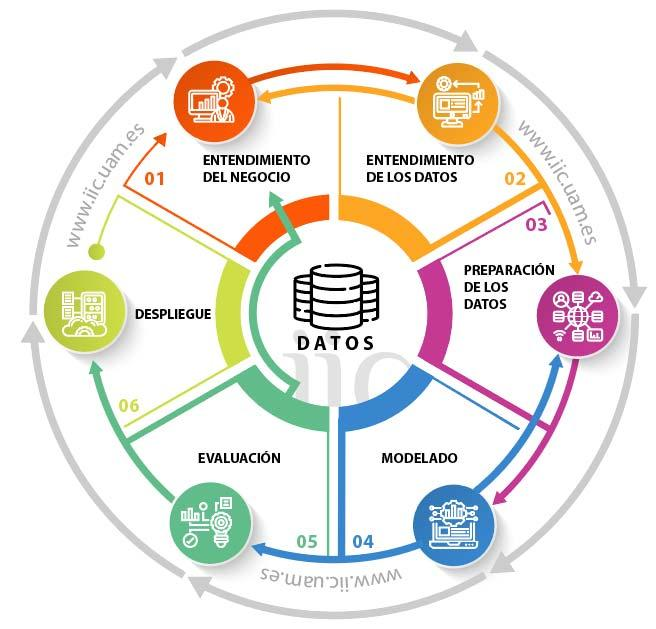
\includegraphics[width=0.55\textwidth]{../Memoria/img/metodologia/crispdm.jpeg}
    \caption{Esquema del ciclo CRISP-DM estándar \cite{haya_crisp_dm}.}
    \label{fig:CRISP-DM}
\end{figure}
    
\end{frame}


\begin{frame}{Fases de CRISP-DM}
      \begin{enumerate}
	      \item Entendimiento del problema.
	      \item Entendimiento de los datos.	      
	      \item Preparación de los datos.
	      \item Modelado.
	      \item Evaluación.
	      \item Despliegue.
      \end{enumerate}
\end{frame}

\section{Entendimiento del problema}
En este capítulo se trata el entendimiento del problema. Tal y como se comenta en el capítulo dos, es la fase inicial de la metología CRISP-DM. A continuación, se alinean los objetivos técnicos con las necesidades del negocio y con el problema a resolver. Se definen requisitos, se identifican métricas de éxito y se trata de dar comprensión sobre el contexto organizacional.


\section{¿Qué es un ataque a un sistema informático?}
Un ataque a un sistema informático constituye una acción deliberada y no autorizada que explota vulnerabilidades con el objetivo de comprometer la confidencialidad, integridad o disponibilidad de los datos y recursos del sistema. Esta actividad maliciosa puede manifestarse a través de diversas técnicas, incluyendo la inyección de código malicioso, la denegación de servicio, el acceso no autorizado y la ingeniería social. Su ejecución busca obtener beneficios ilícitos, interrumpir operaciones o dañar la infraestructura tecnológica.

La consecuencia de un ataque puede variar desde la pérdida o alteración de información sensible hasta la paralización completa de los servicios ofrecidos por el sistema. La identificación, análisis y mitigación de estas amenazas representan un aspecto fundamental en la seguridad informática, requiriendo la implementación de medidas preventivas y reactivas para proteger los activos digitales de una organización o individuo.

\section{Tipos de ataque a sistemas informáticos}


\section{¿Qué es TCP?}

El Protocolo de Control de Transmisión (TCP) constituye uno de los protocolos fundamentales de la capa de transporte del modelo TCP/IP, sobre el cual se sustenta gran parte de la comunicación en redes IP, incluyendo Internet. Su diseño se orienta a proporcionar un servicio de transferencia de datos fiable, ordenado y con detección de errores entre aplicaciones que se ejecutan en sistemas finales diferentes. Para lograr esta fiabilidad, TCP establece una conexión virtual punto a punto entre las aplicaciones comunicantes mediante un proceso de "three-way handshake", lo que permite la negociación de parámetros de la conexión y la sincronización de los números de secuencia iniciales.

\begin{figure}[htbp]
    \centering
    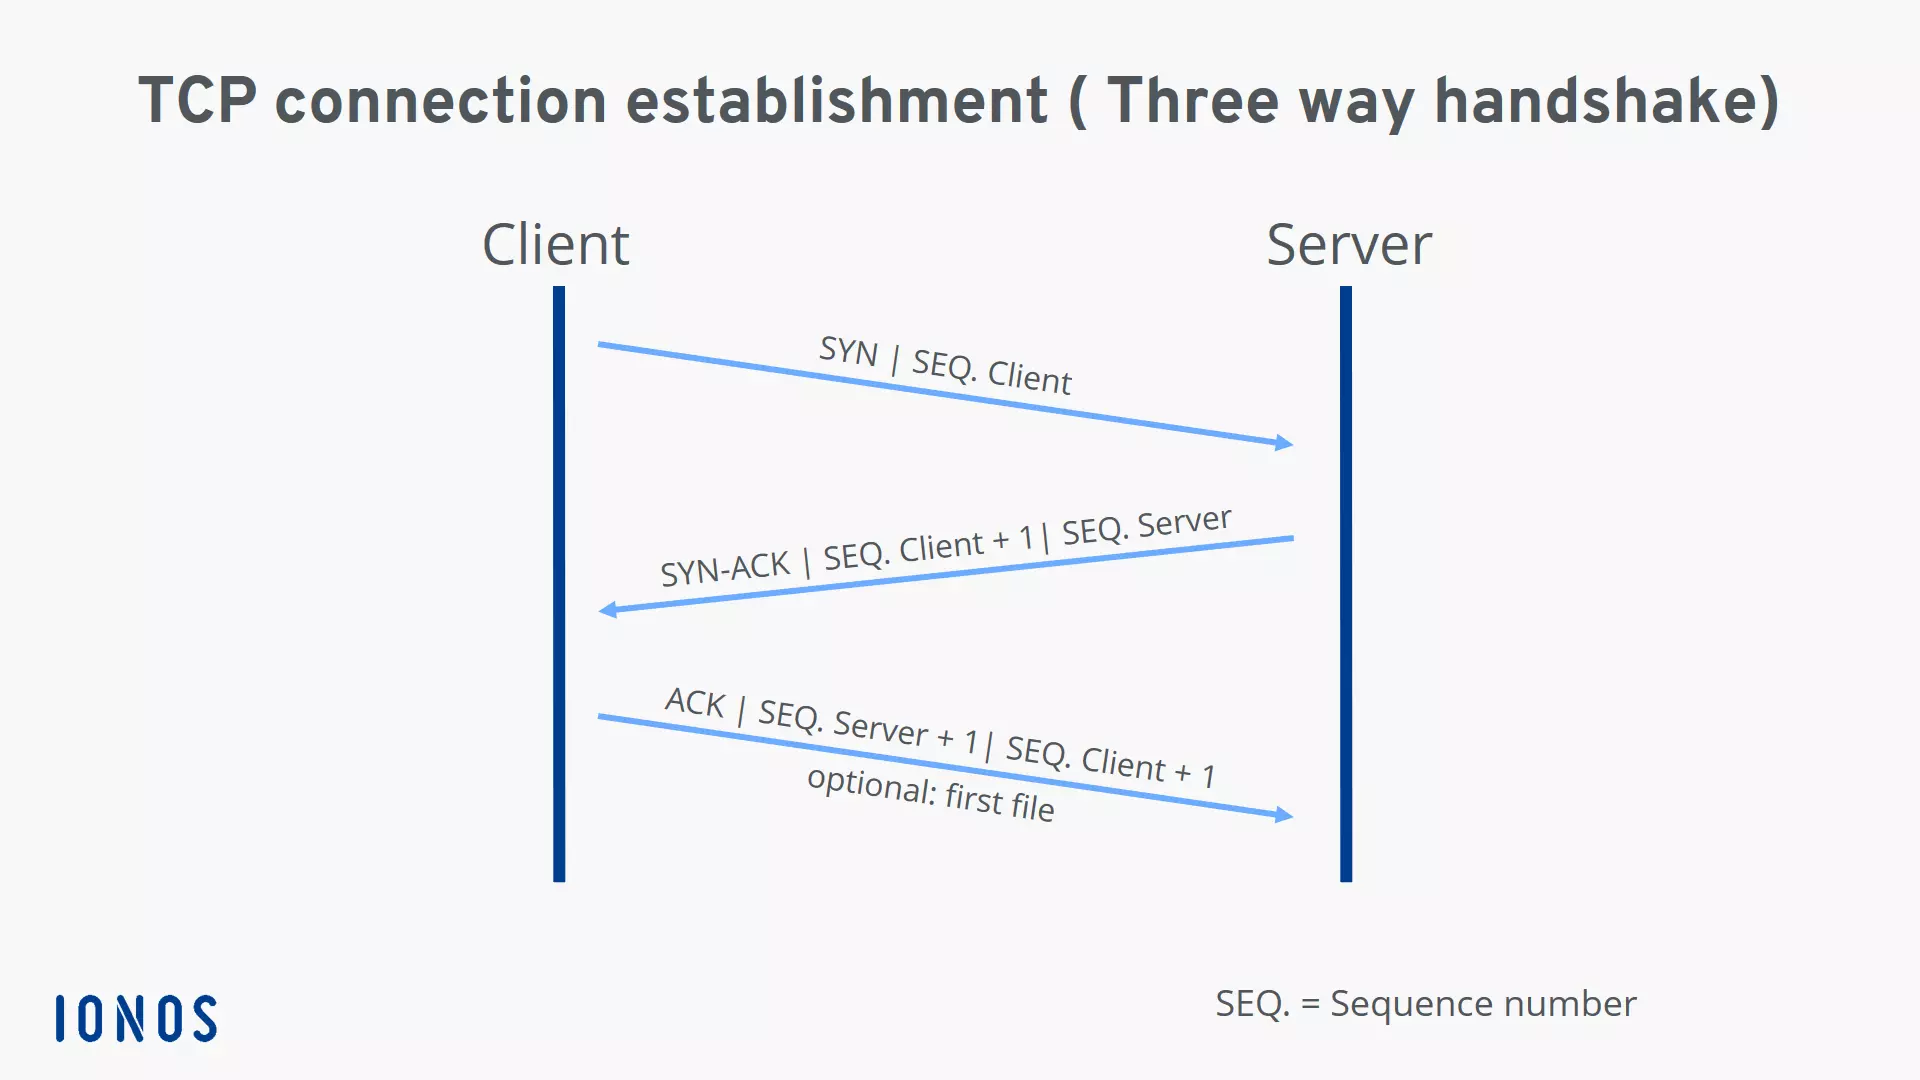
\includegraphics[width=0.8\textwidth]{./img/ent-problema/EsquemaTCP.png}
    \caption{Esquema funcionamiento TCP. \cite{tcpprotocolionos}}
    \label{fig:EsquemaTCP}
\end{figure}

El protocolo garantiza la entrega ordenada de la información al receptor mediante la asignación de números de secuencia a cada byte transmitido, permitiendo así la reordenación en caso de que la información no llegue al receptor en el orden correcto. La fiabilidad se logra a través de un mecanismo de acuse de recibo (acknowledgment, ACK) positivo con retransmisión, donde el receptor confirma la recepción correcta de los paquetes de información, y el emisor retransmite aquellos partes de la información para los que no recibe confirmación dentro de un tiempo límite (timeout).

\subsection{¿Qué es un segmento TCP?}
Una vez establecida la conexión, TCP divide los datos de la aplicación en unidades más pequeñas denominadas segmentos. Un segmento o paquete TCP constituye la unidad de datos fundamental que se intercambia a través de una red utilizando el mencionado protocolo TCP. Este segmento encapsula una porción de los datos de la capa de aplicación, precedida por una cabecera TCP. 

La cabecera TCP contiene información de control esencial para la funcionalidad del protocolo, incluyendo los números de puerto de origen y destino que identifican las aplicaciones comunicantes, los números de secuencia y de acuse de recibo (ACK) que garantizan la entrega ordenada y fiable, las banderas de control que indican el propósito del segmento (establecimiento de conexión, finalización, ACK, entre otros muchos), y otros campos como la ventana de recepción para el control de flujo y la suma de verificación para la detección de errores.


\begin{figure}[htbp]
    \centering
    
\includegraphics[width=0.8\textwidth]{./img/ent-problema/SegmentoTCP.png}
    \caption{Esquema segmento TCP. \cite{tcpsegment}}
    \label{fig:SegmentoTCP}
\end{figure}

En el proceso de transmisión, el segmento TCP se encapsula a su vez dentro de un paquete IP (Protocolo de Internet) para su enrutamiento a través de la red. El paquete IP añade su propia cabecera con las direcciones IP de origen y destino, entre otra información necesaria para el transporte a nivel de red. 

\begin{figure}[htbp]
    \centering
    
\includegraphics[width=0.8\textwidth]{./img/ent-problema/PaqueteIP.png}
    \caption{Formato de la cabecera en IPv4. \cite{paqueteip}}
    \label{fig:PaqueteIP}
\end{figure}

\section{Importancia de protegerse frente a un ataque}

La importancia de protegerse frente a ataques informáticos radica en la salvaguarda de activos digitales críticos, la garantía de la continuidad operativa y la preservación de la confianza y la reputación. En un entorno digital cada vez más interconectado, los ataques informáticos representan una amenaza significativa para individuos, organizaciones y la sociedad en su conjunto, pudiendo acarrear consecuencias devastadoras.

Para las organizaciones, las implicaciones de un ataque informático pueden ser aún más costosas. Estas implicaciones incluyen pérdidas financieras directas debido al robo de fondos, la interrupción de las operaciones comerciales, los costes de recuperación y las posibles sanciones regulatorias. Además, se puede producir un daño significativo a la reputación y la pérdida de la confianza de los clientes, lo que a largo plazo afecta la viabilidad del negocio. Los ataques también pueden resultar en el robo de propiedad intelectual, secretos comerciales e información estratégica, otorgando ventajas competitivas a adversarios. 

Por otra parte, la interrupción de servicios críticos, como energía, comunicaciones o sanidad, puede tener consecuencias graves para la sociedad en su conjunto.

La protección frente a ataques informáticos no es solo una cuestión de seguridad tecnológica, sino una necesidad imperante en la actualidad para proteger activos valiosos, asegurar la continuidad de las actividades, mantener la confianza de los usuarios y garantizar la estabilidad y el bienestar en el mundo digital actual. La implementación de prácticas de seguridad robustas y la concienciación sobre las amenazas cibernéticas son fundamentales en a la hora de defenderse de estos ataques.


\section{Importancia de detectar los ataques rápidamente}

La detección temprana de ataques informáticos constituye un pilar fundamental en la ciberseguridad moderna debido a su capacidad para mitigar consecuencias críticas. Cuando un sistema logra identificar intrusiones o actividades maliciosas en sus fases iniciales, se reducen significativamente los daños operativos y económicos. Esta rapidez de respuesta permite contener amenazas antes de que comprometan infraestructuras completas, preservando tanto la integridad de los datos como la continuidad del negocio.

Desde una perspectiva técnica, la identificación inmediata limita la superficie de ataque, impidiendo que los actores maliciosos escalen privilegios o se propaguen lateralmente por la red. En el ámbito regulatorio, cumple con los estrictos plazos que exigen normativas como el Reglamento General de Protección de Datos (RGPD), que obliga a notificar violaciones de seguridad en un máximo de 72 horas. Además, desde el punto de vista económico, reduce los costes asociados a las reparaciones, que suelen multiplicarse exponencialmente cuando los ataques permanecen indetectados durante largos períodos.


La capacidad de detectar rápidamente anomalías en el tráfico de red, accesos no autorizados o patrones de comportamiento sospechosos no solo protege los activos digitales, sino que también salvaguarda la reputación institucional. Organizaciones con sistemas de detección temprana robustos demuestran proactividad ante clientes y socios comerciales, generando confianza en su capacidad para manejar información sensible. Esta anticipación resulta especialmente crítica en entornos donde la disponibilidad del servicio es primordial, como en las infraestructuras críticas anteriormente mencionadas.

\section{Soluciones comerciales o actuales a estos problemas}

En esta sección se comentan algunas de las soluciones y software que se utilizan en la actualiadad para detectar y neutralizar posibles ataques informáticos. Estas herramientas protegen los sistemas informáticos analizando y controlando el tráfico de la red.

Los firewalls de próxima generación (NGFW) como Palo Alto Networks, Check Point o Cisco Firepower, inspeccionan el tráfico de red a un nivel profundo (Deep Packet Inspection - DPI), analizando el contenido de los paquetes más allá de los puertos y protocolos tradicionales. Esto permite identificar y bloquear amenazas sofisticadas, malware, y tráfico de aplicaciones maliciosas, además de ofrecer funcionalidades como prevención de intrusiones (IPS) y control de aplicaciones. \cite{cosmikal_firewall}

Los sistemas de detección y prevención de intrusiones o IDS e IPS, como: Snort, Suricata o Trend Micro TippingPoint, monitorean el tráfico de red en tiempo real en busca de patrones sospechosos o firmas de ataques conocidos. Los IDS alertan sobre posibles intrusiones, mientras que los IPS tienen la capacidad de bloquear o mitigar activamente el tráfico malicioso detectado, interrumpiendo los ataques en curso. \cite{geekflare_ids_ips}

La microsegmentación de red con herramientas como VMware NSX, Cisco ACI o Illumio, divide la red en segmentos más pequeños y aislados, aplicando políticas de seguridad granular a cada segmento. Esto limita el movimiento lateral de los atacantes dentro de la red una vez que han comprometido un punto inicial. Al controlar el tráfico entre estos segmentos, se reduce la superficie de ataque y se contiene la propagación de las amenazas. \cite{paloaltonetworks_microsegmentation}

\section{Requisitos}  \label{sec.requisitos} 
Como se ha comentado en la sección \ref{sec.objetivos-pro}\nameref{sec.objetivos-pro}, 
el principal objetivo del proyecto es desarrollar un modelo neuronal que detecte la presencia de ataques en una red informática y los clasifique según su tipo. Para cumplir con dicho objetivo, se considera imprescindible cumplir con los requisitos que se listan a continuación.

\subsection{Requisitos Funcionales}   \label{sec.req-funcionales}
\textbf{Primera versión de requisitos, no me convencen mucho}
\begin{itemize}  
    \item \textbf{RF-1}: El sistema deberá detectar cuales de las conexiones podrían ser potenciales intrusiones en la red.
    \item \textbf{RF-2}: El sistema deberá clasificará las conexiones en 10 categorías predefinidas en \nameref{tab:attacks-tab}.  
	\item \textbf{RF-3}: El sistem deberá ser capaz de procesar formatos estándar de logs como son Syslog, NetFlow y PCAP.
	\item \textbf{RF-4}: El sistema deberá diferenciar entre ataques conocidos (basados en firmas) y desconocidos (basados en anomalías).
	\item \textbf{RF-5}: El sistema deberá ofrecer API REST para conexión con SIEMs (Splunk, IBM QRadar)
	\item \textbf{RF-6}: Generar alertas automatizadas con nivel de criticidad (bajo/medio/alto).
	\item \textbf{RF-7}: Proveer recomendaciones de mitigación básicas (ej. bloquear IPs maliciosas)

	
	
\textbf{¿Debería integrar el modelo en algún sistema o crear un script o alguna forma para comunicarme con él?}
		
\end{itemize}  

\subsection{Requisitos No Funcionales}   \label{sec.req-no-funcionales}
\begin{itemize}  
    \item \textbf{RNF-1}: Latencia <50 ms en redes de 10Gbps (requisito crítico para SOC~\cite{nist2021ai}).  
    \item \textbf{RNF-2}: Interfaz accesible para usuarios no técnicos (evaluado con test SUS~\cite{brooke1996sus}).  
\end{itemize}  


\section{Contexto organizacional} \label{sec.contexto-organizacional}


\section{Objetivos del proyecto}

\section{Entendimiento de los datos}
Este capítulo se corresponde con la segunda etapa de la metodología CRISP-DM, En el se explicará la naturaleza de los datos y sus características, así como los valores atípicos que presentan y sus sesgos.

\section{Origen de los datos}  \label{sec.origen-datos}
Los datos que se han utilizado para desarrollar este trabajo, se han obtenido de  conjuntos de datos diseñados para entrenar Sistemas de Detección de Intrusión de Red (NIDS) basados en el aprendizaje automático. El conjunto de datos en cuenstión  forma parte de un análisis realizado en la Universidad de Queensland, Australia \cite{luay2025NetFlowDatasetsV3}.


El \textit{dataset} utilizado es \texttt{NF-UNSW-NB15-v3}, este es una versión basada en NetFlow del conocido conjunto de datos UNSW-NB15, mejorada con características adicionales de NetFlow y etiquetada de acuerdo con sus respectivas categorías de ataque. 

\section{Tipos de ataques registrados en los datos} \label{sec.tipo-ataques}
En esta sección se explican los tipos de datos presentes en el \textit{dataset} que se utiliza para entrenar a los modelos del proyecto. Se explica en que consiste cada tipo de ataque registrado así como el número exacto de ataques de cada tipo presente.

El conjunto de datos consiste en un total de 2\,365\,424 flujos de datos, donde 127\,639 (5,4\%) son muestras de ataque y 2\,237\,731 (94,6\%) son benignos. Los flujos de ataque se clasifican en nueve clases, cada una representando una amenaza a la red distinta. La Tabla \ref{tab:attacks-tab} proporciona una distribución detallada del conjunto de datos:

\begin{table}[H]
\begin{tabular}{|l|c|>{\RaggedRight}p{8cm}|} % Ajusta el ancho (8cm) según necesites
\hline
\rowcolor[HTML]{C0C0C0} 
\textbf{Clase} & \textbf{Cantidad} & \textbf{Descripción} \\ \hline
Benigno & 2\,237\,731 & Flujos normales no maliciosos. \\ \hline
\textit{Fuzzers} & 33\,816 & Tipo de ataque en el que el atacante envía grandes cantidades de datos aleatorios que hacen que un sistema se bloquee y también apuntan a descubrir vulnerabilidades de seguridad en un sistema. \\ \hline
\textit{Analysis} & 2\,381 & Un grupo que presenta una variedad de amenazas que se dirigen a aplicaciones web a través de puertos, correos electrónicos y \textit{scripts}. \\ \hline
\textit{Backdoor} & 1\,226 & Una técnica que tiene como objetivo eludir los mecanismos de seguridad respondiendo a aplicaciones específicas de clientes construidos. \\ \hline
DoS & 5\,980 & La denegación de servicio es un intento de sobrecargar los recursos de un sistema informático con el objetivo de evitar el acceso o la disponibilidad de sus datos. \\ \hline
\textit{Exploits} & 42\,748 & Son secuencias de comandos que controlan el comportamiento de un \textit{host} a través de una vulnerabilidad conocida. \\ \hline
\textit{Generic} & 19\,651 & Un método que se dirige a la criptografía y causa una colisión con cada cifrado de bloques. \\ \hline
\textit{Reconnaissance} & 17\,074 & Una técnica para recopilar información sobre un \textit{host} de red, también se conoce como sonda. \\ \hline
\textit{Shellcode} & 4\,659 & Un \textit{malware} que penetra en un código para controlar el \textit{host} de una víctima. \\ \hline
\textit{Worms} & 158 & Ataques que se replican y se extienden a otros sistemas. \\ \hline
\end{tabular}
\centering
\caption{Clasificación de amenazas de seguridad del dataset \texttt{NF-UNSW-NB15-v3}.} 
\label{tab:attacks-tab}
\end{table}

\section{Parámetros de los datos} \label{sec.param-datos}
En esta sección se explicarán el significado de cada uno de los 55 atributos que componen cada fila del \textit{dataset} seleccionado. El \textit{dataset}, que es de dominio público se puede descargar en formato .csv donde los atributos se encuentran separados por comas \cite{luay2025NetFlowDatasetsV3}.

\begin{enumerate}
    \item \texttt{IPV4\_SRC\_ADDR}: Dirección IPv4 de origen.
    \item \texttt{IPV4\_DST\_ADDR}: Dirección IPv4 de destino.
    \item \texttt{L4\_SRC\_PORT}: Número de puerto de origen de la capa 4.
    \item \texttt{L4\_DST\_PORT}: Número de puerto de destino de la capa 4.
    \item \texttt{PROTOCOL}: Byte identificador del protocolo IP.
    \item \texttt{L7\_PROTO}: Protocolo que opera en la capa 7 del Modelo OSI, también conocida como capa de aplicación.
    \item \texttt{IN\_BYTES}: Número de bytes entrantes.
    \item \texttt{OUT\_BYTES}: Número de bytes salientes.
    \item \texttt{IN\_PKTS}: Número de paquetes entrantes.
    \item \texttt{OUT\_PKTS}: Número de paquetes salientes.
    \item \texttt{FLOW\_DURATION\_MILLISECONDS}: Duración del flujo en ms.
    \item \texttt{TCP\_FLAGS}: \textit{Bits} dentro del encabezado TCP que indican el estado o la dirección de una conexión TCP.
    \item \texttt{CLIENT\_TCP\_FLAGS}: \textit{Bits} dentro del encabezado TCP que indican el estado de la conexión TCP del cliente.
    \item \texttt{SERVER\_TCP\_FLAGS}: \textit{Bits} dentro del encabezado TCP que indican el estado de la conexión TCP del servidor.
    \item \texttt{DURATION\_IN}: Duración del flujo Cliente a Servidor (ms).
    \item \texttt{DURATION\_OUT}: Duración del flujo Cliente a Servidor (ms).
    \item \texttt{MIN\_TTL}: Mínimo valor del TTL (\textit{Time To Live}), que limita la duración de un paquete de datos en una red informática, durante la sesión TCP.
    \item \texttt{MAX\_TTL}: Maximo valor del TTL (\textit{Time To Live}), que limita la duración de un paquete de datos en una red informática, durante la sesión TCP.
    \item \texttt{LONGEST\_FLOW\_PKT}: Paquete de mayor tamaño enviado durante la conexión de los sistemas (bytes).
    \item \texttt{SHORTEST\_FLOW\_PKT}: Paquete de menor tamaño enviado durante la conexión de los sistemas (bytes)
    \item \texttt{MIN\_IP\_PKT\_LEN}: Longitud del paquete IP más pequeño del flujo observado.
    \item \texttt{MAX\_IP\_PKT\_LEN}: Longitud del paquete IP más grande del flujo observado.
    \item \texttt{SRC\_TO\_DST\_SECOND\_BYTES}: \textit{Bytes}/segundo de origen a destino.
    \item \texttt{DST\_TO\_SRC\_SECOND\_BYTES}: \textit{Bytes}/segundo de destino a origen.
    \item \texttt{RETRANSMITTED\_IN\_BYTES}: Número de bytes TCP retransmitidos del flujo (src a dst).
    \item \texttt{RETRANSMITTED\_IN\_PKTS}: Número de paquetes TCP retransmitidos del flujo (src a dst).
    \item \texttt{RETRANSMITTED\_OUT\_BYTES}: Número de bytes TCP retransmitidos del flujo (dst a src).
    \item \texttt{RETRANSMITTED\_OUT\_PKTS}: Número de paquetes TCP retransmitidos del flujo (dst a src).
    \item \texttt{SRC\_TO\_DST\_AVG\_THROUGHPUT}: Tasa de transferencia promedio de origen a destino (bps).
    \item \texttt{DST\_TO\_SRC\_AVG\_THROUGHPUT}: Tasa de transferencia promedio de destino a origen (bps).
    \item \texttt{NUM\_PKTS\_UP\_TO\_128\_BYTES}: Paquetes cuyo tamaño IP es $ \leq $ 128.
    \item \texttt{NUM\_PKTS\_128\_TO\_256\_BYTES}: Paquetes cuyo tamaño IP es  $ > $ 128 y $ \leq $ 256.
    \item \texttt{NUM\_PKTS\_256\_TO\_512\_BYTES}: Paquetes cuyo tamaño IP es $ > $ 256 y $ \leq $ 512.
    \item \texttt{NUM\_PKTS\_512\_TO\_1024\_BYTES}: Paquetes cuyo tamaño IP es $ > $ 512 y $ \leq $ 1024.
    \item \texttt{NUM\_PKTS\_1024\_TO\_1514\_BYTES}: Paquetes cuyo tamaño IP es $ > $ 1024 y $ \leq $ 1514.
    \item \texttt{TCP\_WIN\_MAX\_IN}: Ventana TCP máxima (src a dst).
    \item \texttt{TCP\_WIN\_MAX\_OUT}: Ventana TCP máxima (dst a src).
    \item \texttt{ICMP\_TYPE}: Tipo ICMP * 256 + Código ICMP.
    \item \texttt{ICMP\_IPV4\_TYPE}: Tipo ICMP.
    \item \texttt{DNS\_QUERY\_ID}: ID de transacción de la consulta DNS.
    \item \texttt{DNS\_QUERY\_TYPE}: Tipo de consulta DNS (ej., 1=A, 2=NS..).
    \item \texttt{DNS\_TTL\_ANSWER}: TTL del primer registro A (si existe).
    \item \texttt{FTP\_COMMAND\_RET\_CODE}: Código de retorno del comando del cliente FTP.
    \item \texttt{FLOW\_START\_MILLISECONDS}: Marca de tiempo de inicio del flujo en ms.
    \item \texttt{FLOW\_END\_MILLISECONDS}: Marca de tiempo de fin del flujo en ms.
    \item \texttt{SRC\_TO\_DST\_IAT\_MIN}: IAT mínimo (src a dst).
    \item \texttt{SRC\_TO\_DST\_IAT\_MAX}: IAT máximo (src a dst).
    \item \texttt{SRC\_TO\_DST\_IAT\_AVG}: IAT promedio (src a dst).
    \item \texttt{SRC\_TO\_DST\_IAT\_STDDEV}: Desviación estándar del IAT (src a dst).
    \item \texttt{DST\_TO\_SRC\_IAT\_MIN}: IAT mínimo (dst a src).
    \item \texttt{DST\_TO\_SRC\_IAT\_MAX}: IAT máximo (dst a src).
    \item \texttt{DST\_TO\_SRC\_IAT\_AVG}: IAT promedio (dst a src).
    \item \texttt{DST\_TO\_SRC\_IAT\_STDDEV}: Desviación estándar del IAT (dst a src).
\end{enumerate}

Este conjunto de datos ya se encontraba previamente etiquetado, lo que permite realizar un trabajo como el propuesto en el tiempo establecido. Típicamente, los conjuntos de datos enfocados a la clasificación suelen tener una única etiqueta, pero este conjunto de datos tiene dos, lo que agiliza el tratamiento del conjunto de los datos para el entrenamiento y la evaluación de los modelos que se proponen en este proyecto.

\begin{enumerate}
    \item \texttt{Label}: Toma valor 0 si el flujo es benigno y 1 si se trata de un ataque.
    \item \texttt{Attack}: Clase de flujo, perteneciente a las clases mencionadas en \ref{tab:attacks-tab} \nameref{tab:attacks-tab}
\end{enumerate}

\section{Selección de atributos}\label{sec:selectdatos}
En esta sección se comentan los atributos prelinimares, así como los valores y los sesgos presentes en el \textit{dataset}. La identificación de estas irregularidades es fundamental para el correcto desarrollo del proyecto.

Al analizar los datos originales del \textit{dataset}, se encuentran características que afectan de forma negativa al entrenamiento del modelo y por lo tanto, a su correcto funcionamiento. A continuación, se mencionan cuales son las características problematicas de los datos que se utilizan.


Tras estudiar los datos, se descubre que algunos parámetros presentan valores infinitos, estos valores alteran la distribución inherente de las variables, introduciendo valores que no se pueden tratar en el proceso de aprendizaje. Los algoritmos de entrenamiento, diseñados para operar con valores numéricos finitos, pueden comportarse de manera impredecible o inestable ante la presencia de infinitos, dificultando la convergencia hacia una solución óptima. Asimismo, la interpretación de las características con valores infinitos se vuelve ambigua, comprometiendo la capacidad del modelo para establecer relaciones significativas con otras variables y para generalizar correctamente a datos futuros que no contengan tales valores extremos. En consecuencia, la presencia de infinitos puede degradar sustancialmente el rendimiento y la fiabilidad del modelo entrenado.

Como se comenta en la sección anterior \ref{sec.param-datos} \nameref{sec.param-datos}, existen dos parámetros que registran la IP origen y la IP destino de la conexión. En principio, si los datos no fuesen sintéticos, la dirección IP de la máquina que origina la comunicación sería aleatoria. En este conjunto de datos, se puede observar como todos los ataques provienen de IP con máscara 175.45.176.255, lo que no encaja con la realiadad. Independientemente de este patrón, que no se manifiesta de forma natural en las conexiones entre sistemas, el uso de las IPs de las máquinas en el entranamiento de los modelos provoca que el algoritmo encargado de este entrenamiento asigne pesos de manera incorrecta a un parámetro que no influye en la clasificación que se propone para este trabajo.



\section{Preparación de los datos}\label{sec.prep-datos}
En esta sección se modificarán los datos que presentan patrones, valores atípicos o sesgos que se comentan en la sección anterior, \ref{sec:selectdatos} \nameref{sec:selectdatos}. Así como el tratamiento necesario de los datos para poder entrenar los modelos.

Una de las características problemáticas, es la existencia de parámetros con valores infinito. Para tratar con esta problemática existen dos enfoques, o bien se sustituyen los valores infinitos por el máximo valor posible para ese parámetro, o bien, se elimina el flujo al que pertenece cada valor infinito. Para este trabajo, se opta por eliminar los registros con valores infinitos, ya que asginarles un valor falso, podría crear una relación sintética entre los datos y provocar que el modelo no converja en una solución real.

Para entrenar un modelo es necesario que en primer lugar todos los parámetros sean numéricos. En los datos originales del \textit{dataset}, se encuentran tres parámetros que no presentan un formato numérico: \texttt{IPV4\_SRC\_ADDR}, \texttt{IPV4\_DST\_ADDR} y \texttt{Attack}.

\begin{itemize}
	\item Para dar un formato correcto al parámetro \texttt{Attack}, se utiliza el codificador \texttt{LabelEncoder} de la biblioteca sklearn.preprocessing y el método \texttt{fit\_transform} de la biblioteca \texttt{sklearn}. La primera función, \texttt{LabelEncoder} codifica las etiquetas de características categóricas en valores numéricos entre 0 y el número de clases menos 1. Una vez se instancian las categorías del parámtero, el método \texttt{fit\_transform} permite entrenar el codificador y transformar el conjunto de datos en un único paso.
	\item Las direcciones IPv4 están formadas por 4 octetos separados por puntos. Obviamnete este formato no es numérico, por ese motivo se opta por dividir las direcciones IPv4 en 4 parámetros diferentes, uno por cada octeto. De esta manera, si el valor de un flujo para el parámetro \texttt{IPV4\_SRC\_ADDR} es 175.45.176.23, se separa en cuatro nuevos valores que son: 175, 45, 176 y 23. Para realizar esta transformación se utiliza la función \ref{fig:funIPv4} \nameref{fig:funIPv4}.
\begin{figure}[H]
    \centering
    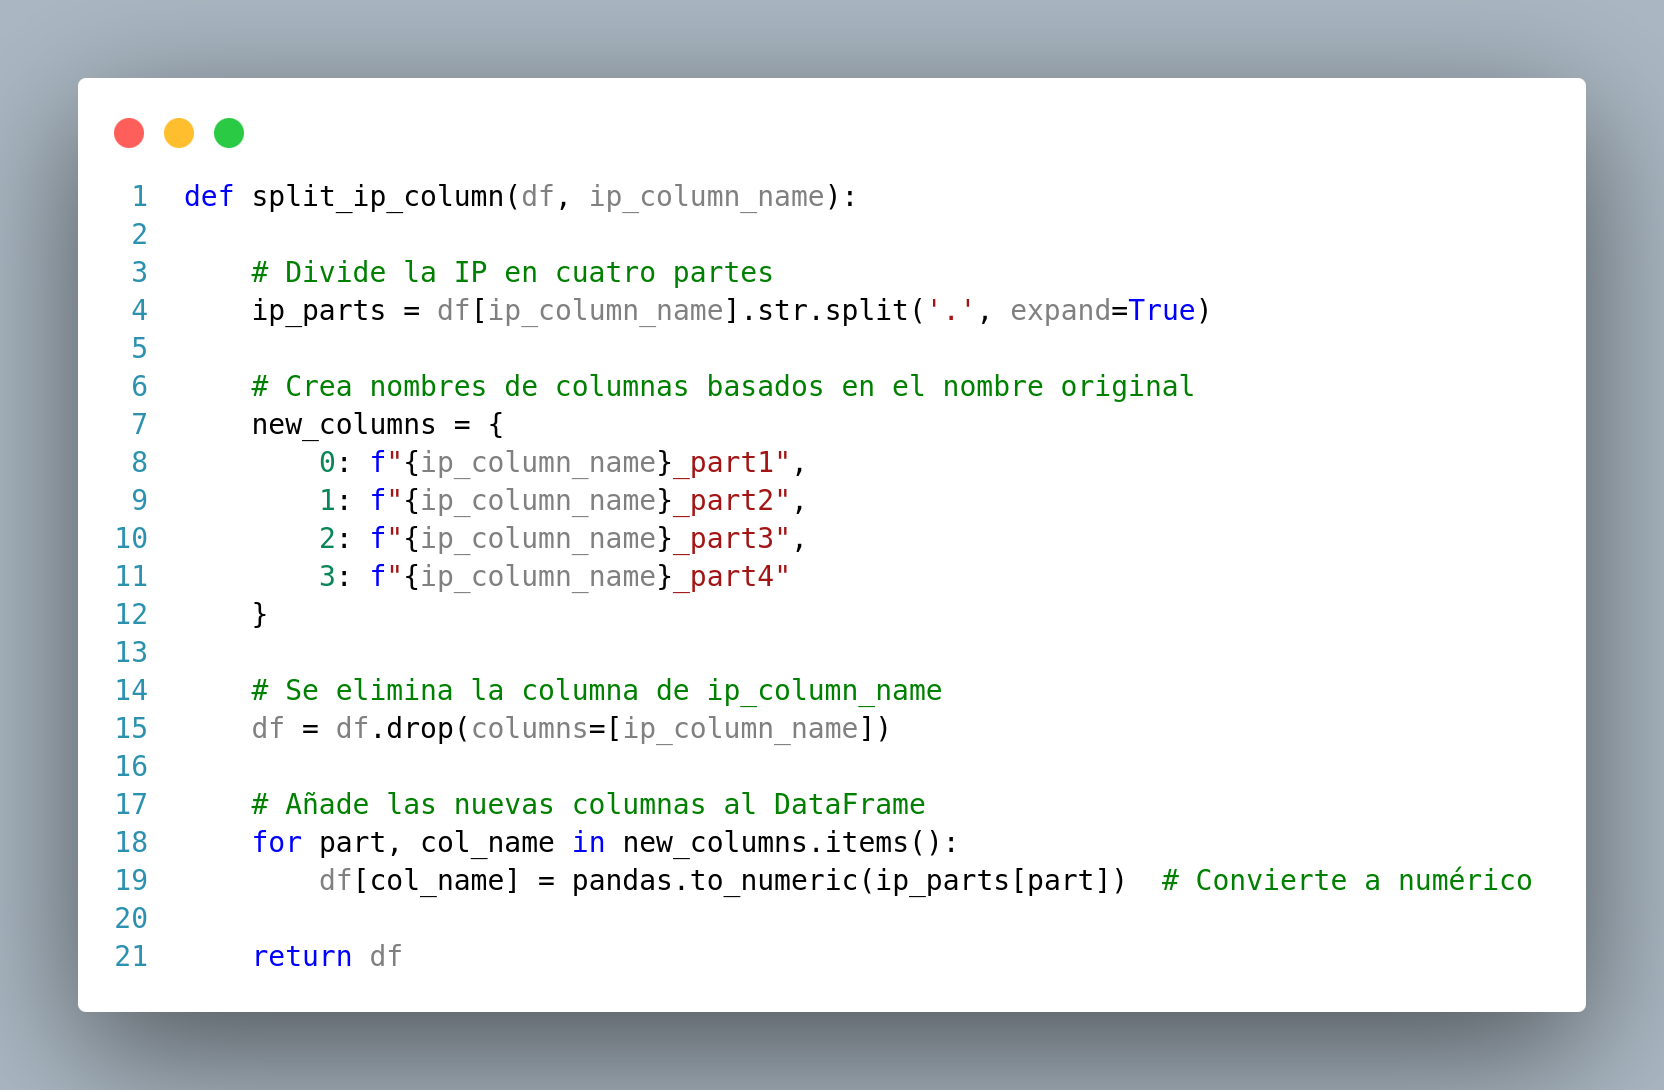
\includegraphics[width=0.8\textwidth]{./img/ent-datos/funIPv4.png}
    \caption{Función de transformación para los parámetros IPv4.}
    \label{fig:funIPv4}
\end{figure}

\end{itemize}

Una vez que todos los parámetros presentan valores numéricos, se separan los parámetros ente los que formarán parte de la entrada del modelo neuronal como atributos (a partir de ahora se les menciona como X) y los que contienen el valor de la salida que debe proporcionar el modelo neuronal llamados etiquetas(a partir de ahora se les menciona como Y).

Los parámetros que pertenecen a Y son \texttt{Label} y \texttt{Attack}. Sin embargo, en función del modelo que se entrena se utiliza o bien \texttt{Label}, o bien \texttt{Attack}, pero nunca los dos al mismo tiempo.

Por su parte, X la conforman el total de los parámetros del \textit{dataset} a excepción de:
\begin{itemize}
	\item \textbf{\texttt{Label} y \texttt{Attack}}: Se trata de los parámetros que conforman Y o etiquetas, si estos parámetros formasen parte de los datos de entrada del modelo, el algoritmo encargado de entrenarlo, les asignaría a estos parámetros unos pesos muy elevados y tendría una tasa teórica de éxito del 100\%, puesto que, se estaría introduciendo la respuesta al problema que se aborda directamente como entrada al modelo. En un sistema informático real esta práctica es imposible.
	\item \textbf{\texttt{IPV4\_SRC\_ADDR} y \texttt{IPV4\_DST\_ADDR}}: Tal y como se menciona en la sección \ref{sec.param-datos} \nameref{sec.param-datos}, estos parámetros presentan un patrón irregular y sintético. Al introducir estos parámetros como entradas para el entrenamiento del modelo, de forma análoga a como sucede con los parámetros \texttt{Label} y \texttt{Attack} se estarían introduciendo valores que no se pueden obtener en una situación realista y condicionando el comportamiento del modelo. Esto implica como se menciona en los siguiente capítulos que el modelo resultante obtendría muy buenas métricas en validación pero muy malas al someterlo a datos que nunca ha visto durante su entrenamiento.
	\item \textbf{\texttt{FLOW\_START\_MILLISECONDS} y \texttt{FLOW\_END\_MILLISECONDS}}: A diferencia de los anteriores parámetros, estos muestran valores que puedan condicionar el entrenamiento de los modelos ni sus resultados, pero se trata de parámetros que ofrecen información redundante, pues el parámetro \texttt{FLOW\_DURATION\_MILLISECONDS} es combinación lineal de estos dos. Al eliminar estos parámetros se agiliza el entrenamiento del modelo y su tiempo de respuesta una vez entrenado sin perjudicar su precisión.
\end{itemize}

Como el conjunto de datos original presentaba 53 atributos de entrada a los modelos y se ha descartado el uso de 4 de ellos, los modelos serán entrenados con 49 atributos de entrada. 

Para finalizar con el tratamiento de los datos, se normalizan los valores de X para que no haya tanta varianza entre los parámetros que lo conforman. Para normalizar los valores se utiliza el escalador \texttt{MinMaxScaler} que forma parte de la biblioteca \texttt{sklearn.preprocessing} junto con el método \texttt{fit\_transform} que se menciona en la explicación de la transformación del parámetro \texttt{Attack}. Llamando a \texttt{MinMaxScaler} con un rango (0,1), tras haber tratado los datos con el método \texttt{fit\_transform}, se obtienen valores escalados en un rango entre 0 y 1, lo que facilita la comparación y el procesamiento por parte de los algoritmos de aprendizaje automático sin alterar las relaciones proporcionales inherentes en los datos originales.


\section{Modelado}
\subsection{Origen de los modelos neuronales}
\begin{frame}{Origen de los modelos neuronales}
	\begin{itemize}
      	\item Ramón y Cajal
      	\item McCulloch/Pitts
      	\item Rosenblatt
    \end{itemize}
    
    \begin{figure}
    \centering
		    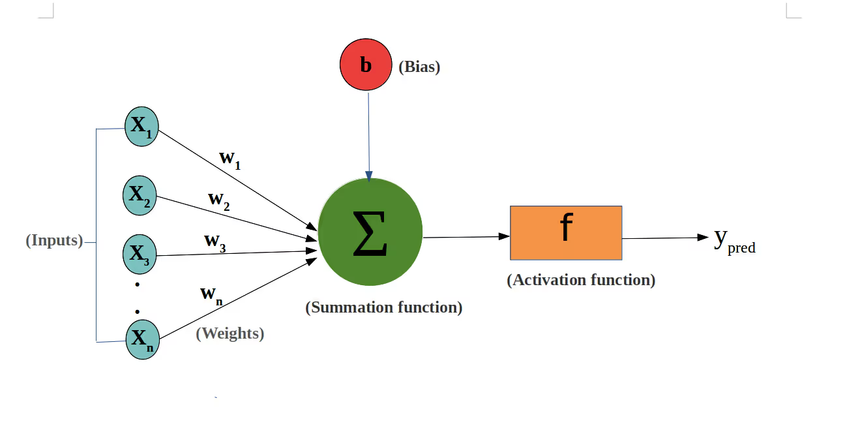
\includegraphics[width=\linewidth]{../Memoria/img/modelo/neuronaartificial.png}
		    \caption{Esquema del funcionamiento de una neurona artificial.}
		    \label{fig:neu-art}
    \end{figure}
      
%    	\begin{figure}[H]
%	    \centering
%	    \hbox{
%	    \begin{minipage}[b]{0.25\textwidth}
%	    		\centering
%		    \includegraphics[width=\linewidth]{./img/RyC.png}
%		    \caption{Ramón y Cajal.}
%		    \label{fig:RyC}
%	    \end{minipage}
%	    
%	    \hspace{1cm}
%	        
%	    \begin{minipage}[b]{0.65\textwidth}
 %   			\centering
%		    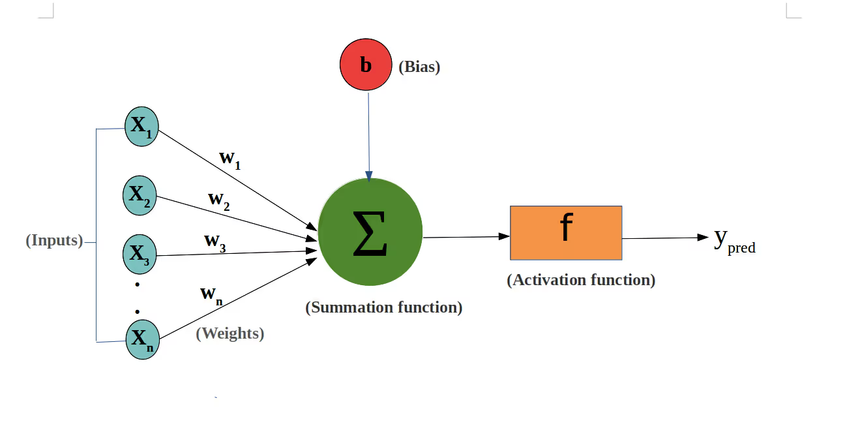
\includegraphics[width=\linewidth]{../Memoria/img/modelo/neuronaartificial.png}
%		    \caption{Esquema del funcionamiento de una neurona artificial 	%	\cite{tomorrow2023peso}.}
%		    \label{fig:neu-art}
%	    \end{minipage}	
%	    }
%	\end{figure}
	
\end{frame}



\begin{frame}{Parámetros e hiperparámetros}

\begin{itemize}

	\item Los parámetros se ajustan a través del algoritmo de optimización, utilizando los cálculos de la función de pérdida durante la fase de entrenamiento de los modelos. Los parámetros de una red neuronal son:
\begin{itemize}
	\item Pesos.
	\item Bias o sesgos.
\end{itemize}
	
	\item Los hiperparámetros son valores que se configuran antes de la fase de entrenamiento y son los responsables de controlar el comportamiento del proceso de entrenamiento. Algunos de los hiperparámetros más importantes son:
\begin{itemize}
	\item Tasa de aprendizaje (\textit{Learning rate}).
	\item Épocas (\textit{Epochs}).
	\item Tamaño de lote (\textit{Batch size}).
\end{itemize}

\end{itemize}
\end{frame}


\subsection{Clasificación con redes neuronales}
\begin{frame}{Matrices de confusión para el MCB}
\begin{itemize}
	\item \small Verdaderos positivos (VP).
    \item \small Falsos positivos (FP).
    \item \small Falsos negativos (FN).
    \item \small Verdaderos negativos (VN).
\end{itemize}

\begin{table}[H]
\centering
\begin{tabular}{|l|c|c|}
\hline
 & \textbf{Predicción Positiva} & \textbf{Predicción Negativa} \\ \hline
\textbf{Real Positivo} & VP & FN \\ \hline
\textbf{Real Negativo} & FP & VN \\ \hline
\end{tabular}
\caption{Matriz de confusión para modelos de clasificación binaria.}
\label{tab:confusion_matrix}
\end{table}
\end{frame}

\begin{frame}{Matriz de confusión para el MCM}
\begin{table}[H]
\centering
\resizebox{\textwidth}{!}{
\begin{tabular}{|>{\raggedright\arraybackslash}m{2.6cm}|*{9}{>{\centering\arraybackslash}m{2cm}|}}
\hline
  & \textbf{Predicción Clase 1} & \textbf{Predicción Clase 2} & \textbf{Predicción Clase 3} & \textbf{Predicción Clase 4} & \textbf{Predicción Clase 5} & \textbf{Predicción Clase 6} & \textbf{Predicción Clase 7} & \textbf{Predicción Clase 8} & \textbf{Predicción Clase 9} \\ \hline
\textbf{Real Clase 1} & \cellcolor{green!20}VP$_{1}$ & FP$_{12}$ & FP$_{13}$ & FP$_{14}$ & FP$_{15}$ & FP$_{16}$ & FP$_{17}$ & FP$_{18}$ & FP$_{19}$ \\ \hline
\textbf{Real Clase 2} & FP$_{21}$ & \cellcolor{green!20}VP$_{2}$ & FP$_{23}$ & FP$_{24}$ & FP$_{25}$ & FP$_{26}$ & FP$_{27}$ & FP$_{28}$ & FP$_{29}$ \\ \hline
\textbf{Real Clase 3} & FP$_{31}$ & FP$_{32}$ & \cellcolor{green!20}VP$_{3}$ & FP$_{34}$ & FP$_{35}$ & FP$_{36}$ & FP$_{37}$ & FP$_{38}$ & FP$_{39}$ \\ \hline
\textbf{Real Clase 4} & FP$_{41}$ & FP$_{42}$ & FP$_{43}$ & \cellcolor{green!20}VP$_{4}$ & FP$_{45}$ & FP$_{46}$ & FP$_{47}$ & FP$_{48}$ & FP$_{49}$ \\ \hline
\textbf{Real Clase 5} & FP$_{51}$ & FP$_{52}$ & FP$_{53}$ & FP$_{54}$ & \cellcolor{green!20}VP$_{5}$ & FP$_{56}$ & FP$_{57}$ & FP$_{58}$ & FP$_{59}$ \\ \hline
\textbf{Real Clase 6} & FP$_{61}$ & FP$_{62}$ & FP$_{63}$ & FP$_{64}$ & FP$_{65}$ & \cellcolor{green!20}VP$_{6}$ & FP$_{67}$ & FP$_{68}$ & FP$_{69}$ \\ \hline
\textbf{Real Clase 7} & FP$_{71}$ & FP$_{72}$ & FP$_{73}$ & FP$_{74}$ & FP$_{75}$ & FP$_{76}$ & \cellcolor{green!20}VP$_{7}$ & FP$_{78}$ & FP$_{79}$ \\ \hline
\textbf{Real Clase 8} & FP$_{81}$ & FP$_{82}$ & FP$_{83}$ & FP$_{84}$ & FP$_{85}$ & FP$_{86}$ & FP$_{87}$ & \cellcolor{green!20}VP$_{8}$ & FP$_{89}$ \\ \hline
\textbf{Real Clase 9} & FP$_{91}$ & FP$_{92}$ & FP$_{93}$ & FP$_{94}$ & FP$_{95}$ & FP$_{96}$ & FP$_{97}$ & FP$_{98}$ & \cellcolor{green!20}VP$_{9}$ \\ \hline
\end{tabular}
}
\caption{Matriz de confusión para los modelos de clasificación multiclase.}
\label{tab:confusion_matrix_9class}
\end{table}
\end{frame}


\subsection{Arquitecturas desarrolladas}
\begin{frame}{Arquitecturas desarrolladas para el MCB}
\begin{itemize}

	\item \textbf{MCB25}: Número de neuronas en la capa oculta igual a la mitad del número de atributos o entradas que recibe el modelo.
	\item \textbf{MCB49}: Número de neuronas en la capa oculta igual al mismo número de atributos o entradas que recibe el modelo.
	\item \textbf{MCB98}: Número de neuronas en la capa oculta igual al doble del número de atributos o entradas que recibe el modelo. 

\end{itemize}

    	\begin{figure}[H]
	    \centering
	    \hbox{
	    \begin{minipage}{0.3\textwidth}
	    		\centering
		    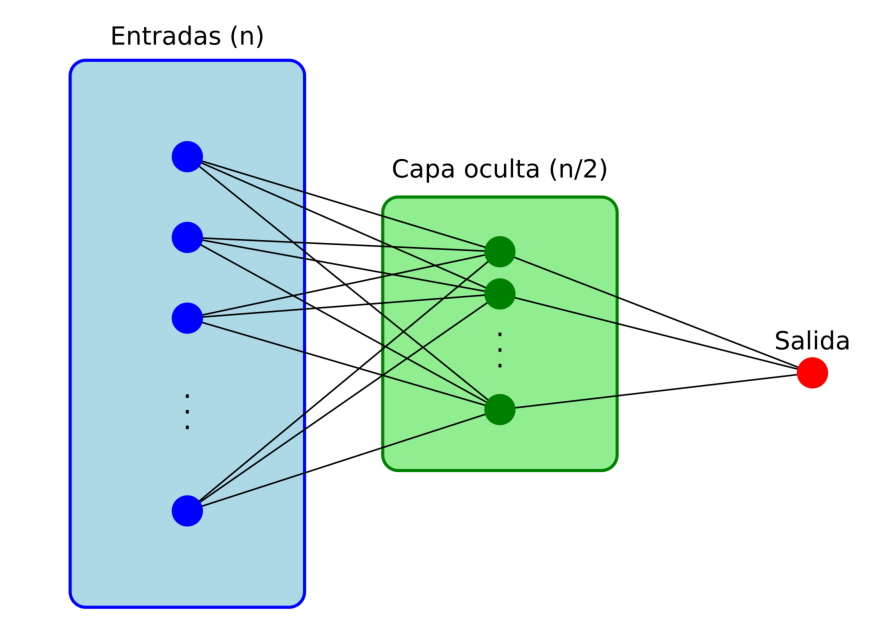
\includegraphics[width=\linewidth]{../Memoria/img/modelo/arquitecturas/arqnmediosBIN.pdf}
    \caption{MCB25.}
	    \end{minipage}
	    
	    \hspace{.5cm}
	        
	    \begin{minipage}{0.3\textwidth}
    			\centering
		    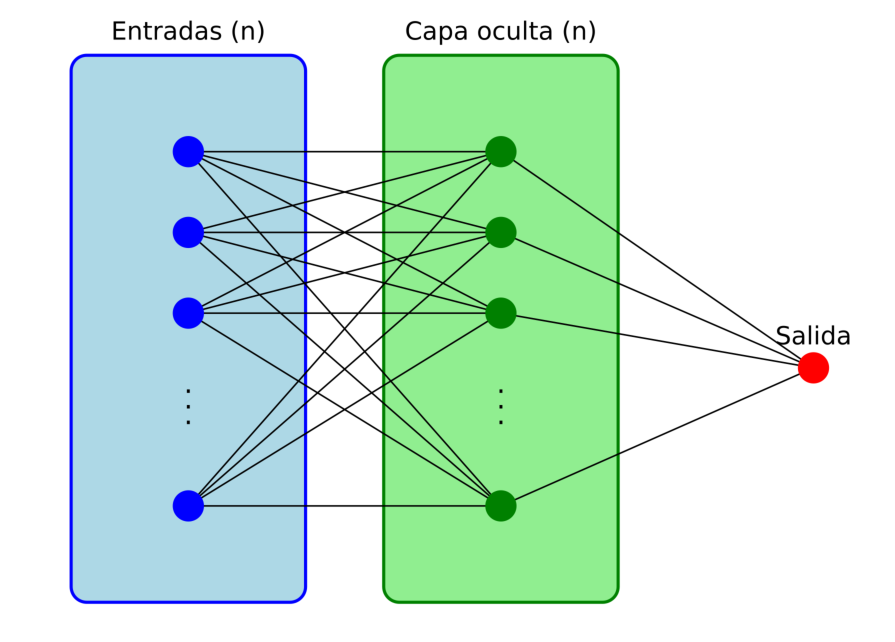
\includegraphics[width=\linewidth]{../Memoria/img/modelo/arquitecturas/arqnBIN.pdf}
		    \caption{MCB49.}
	    \end{minipage}	
	    \hspace{.5cm}
	        
	    \begin{minipage}{0.3\textwidth}
    			\centering
		    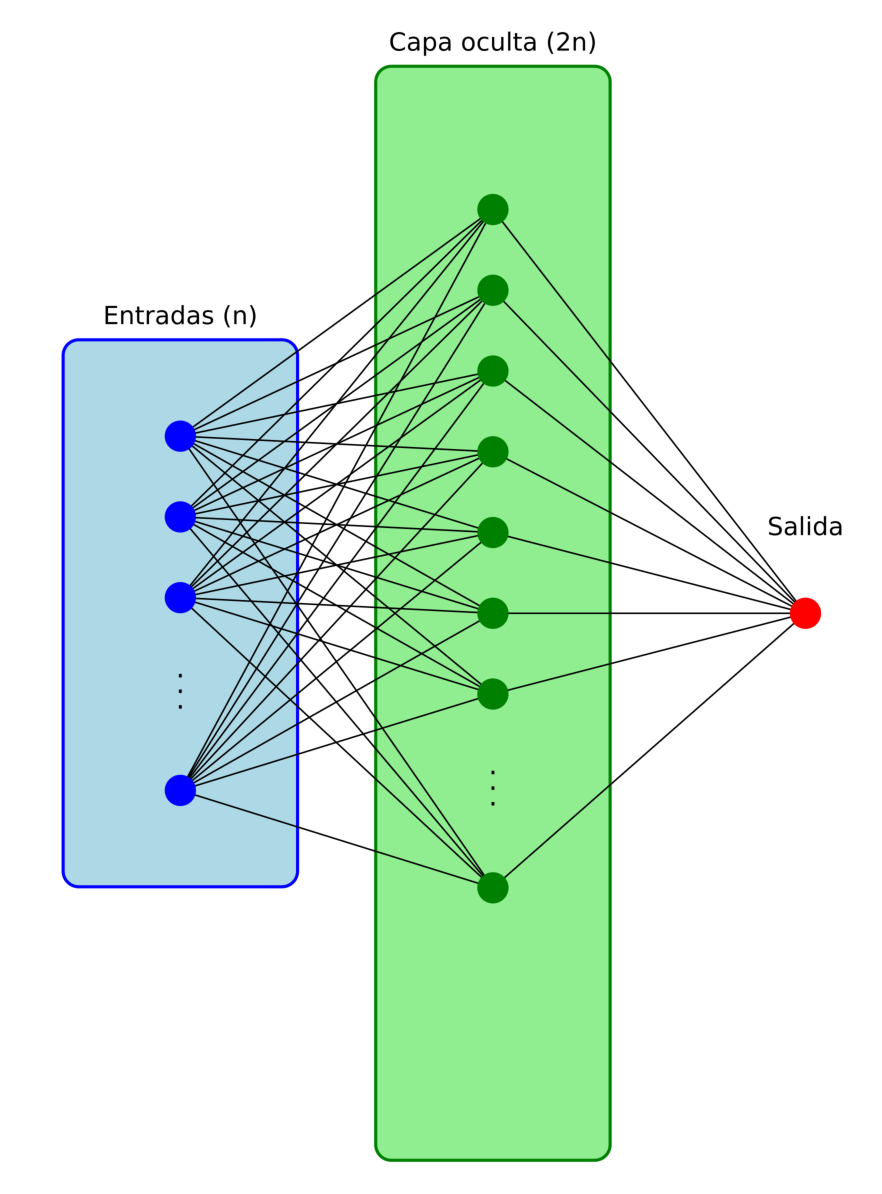
\includegraphics[width=\linewidth]{../Memoria/img/modelo/arquitecturas/arqnnBIN.pdf}
		    \caption{MCB98.}
	    \end{minipage}
	    }
	\end{figure}
	
\end{frame}


\begin{frame}{Arquitecturas desarrolladas para el MCM}
\begin{itemize}


	\item \textbf{MCM25}: Número de neuronas en la capa oculta igual a la mitad del número de atributos o entradas que recibe el modelo.
	\item \textbf{MCM49}: Número de neuronas en la capa oculta igual al mismo número de atributos o entradas que recibe el modelo.
	\item \textbf{MCM98}: Número de neuronas en la capa oculta igual al doble del número de atributos o entradas que recibe el modelo.
\end{itemize}
    	\begin{figure}[H]
	    \centering
	    \hbox{
	    \begin{minipage}{0.3\textwidth}
	    		\centering
		    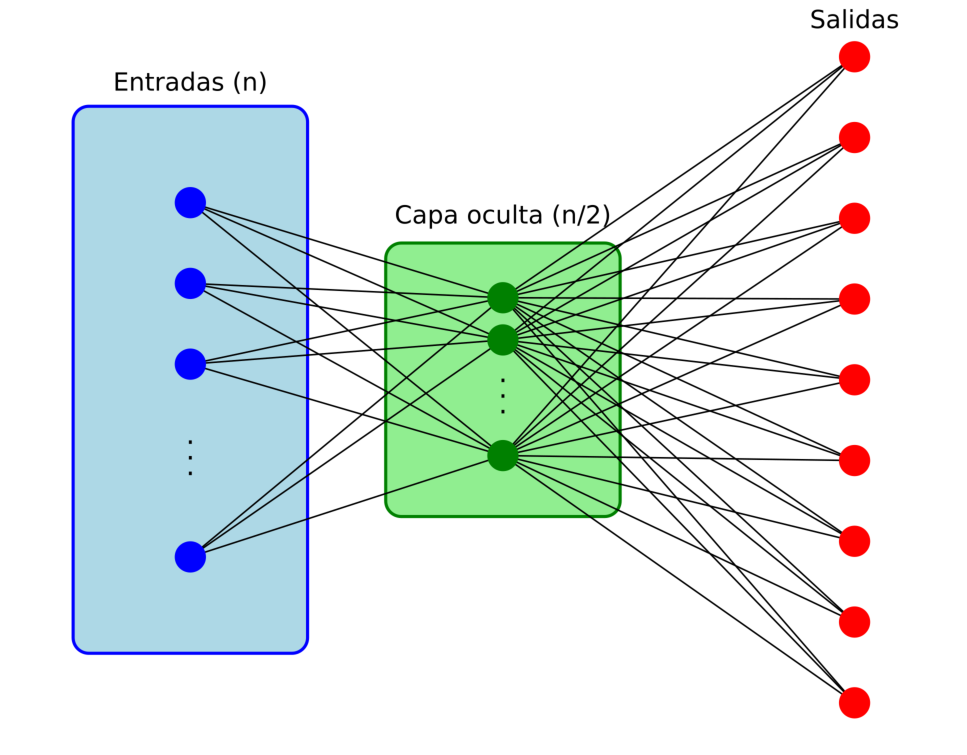
\includegraphics[width=\linewidth]{../Memoria/img/modelo/arquitecturas/arqnmediosMUL.pdf}
    \caption{MCM25.}
	    \end{minipage}
	    
	    \hspace{.5cm}
	        
	    \begin{minipage}{0.3\textwidth}
    			\centering
		    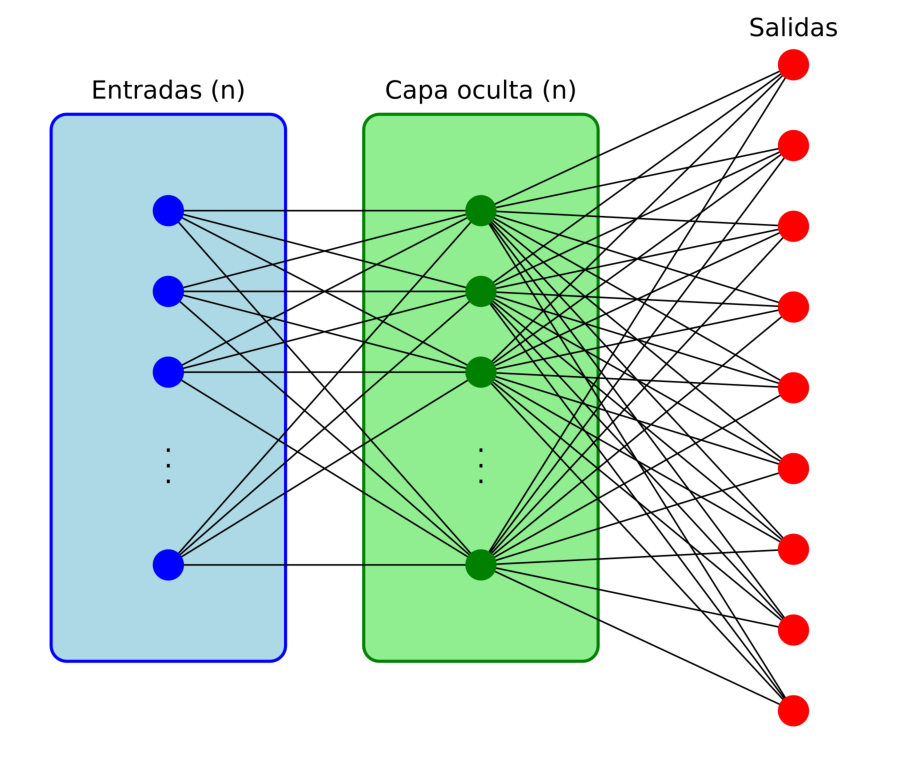
\includegraphics[width=\linewidth]{../Memoria/img/modelo/arquitecturas/arqnMUL.pdf}
		    \caption{MCM49.}
	    \end{minipage}	
	    \hspace{.5cm}
	        
	    \begin{minipage}{0.3\textwidth}
    			\centering
		    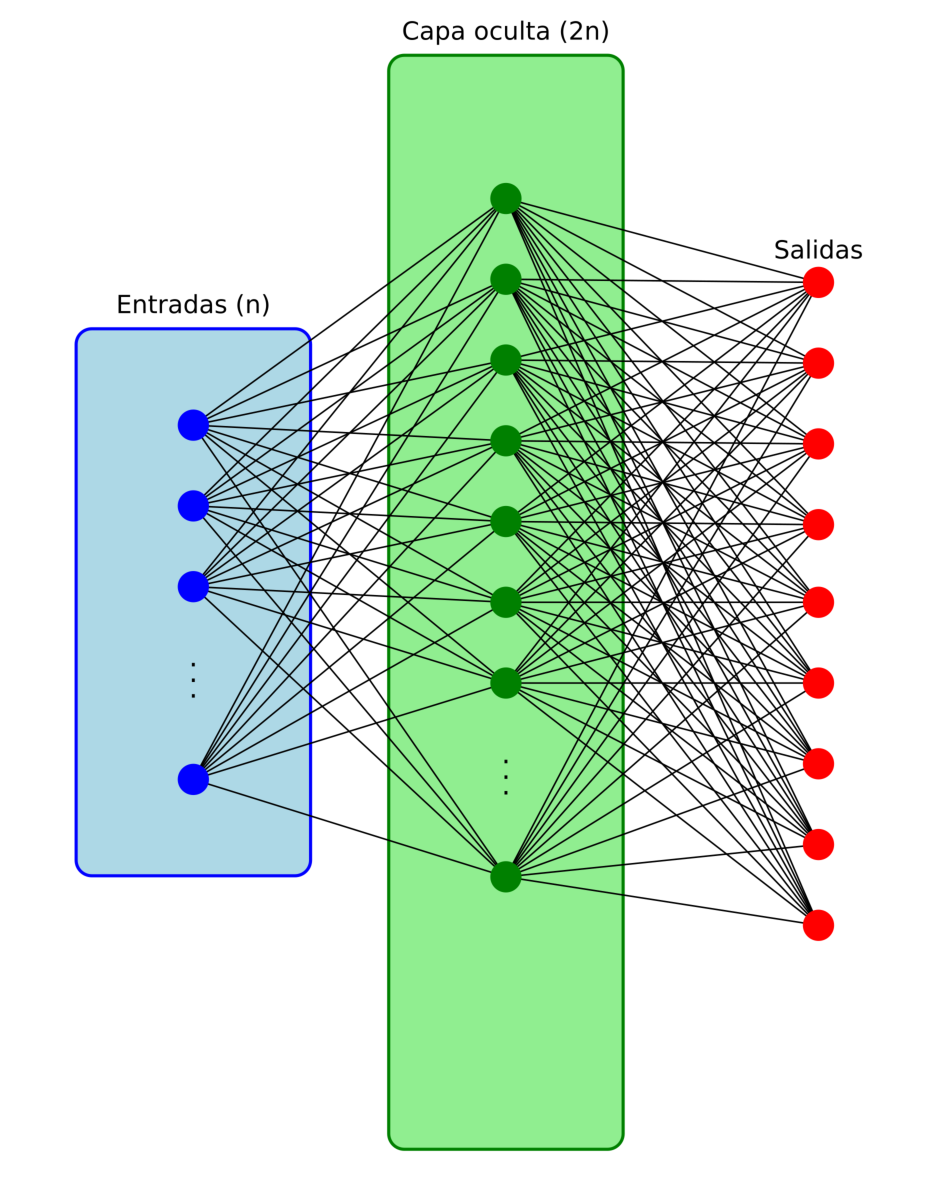
\includegraphics[width=\linewidth]{../Memoria/img/modelo/arquitecturas/arqnnMUL.pdf}
		    \caption{MCM98.}
	    \end{minipage}
	    }
	\end{figure}
	
\end{frame}

\subsection{Implementación de los modelos}
\begin{frame}{Implementación del MCB}
	\begin{itemize}
		\item \textbf{Función de pérdida}: \texttt{BCEWithLogistLoss}
		\item \textbf{Algoritmo de optimización}: \texttt{AdamW}
	\end{itemize}
	
	\begin{figure}[H]
	    \centering
	    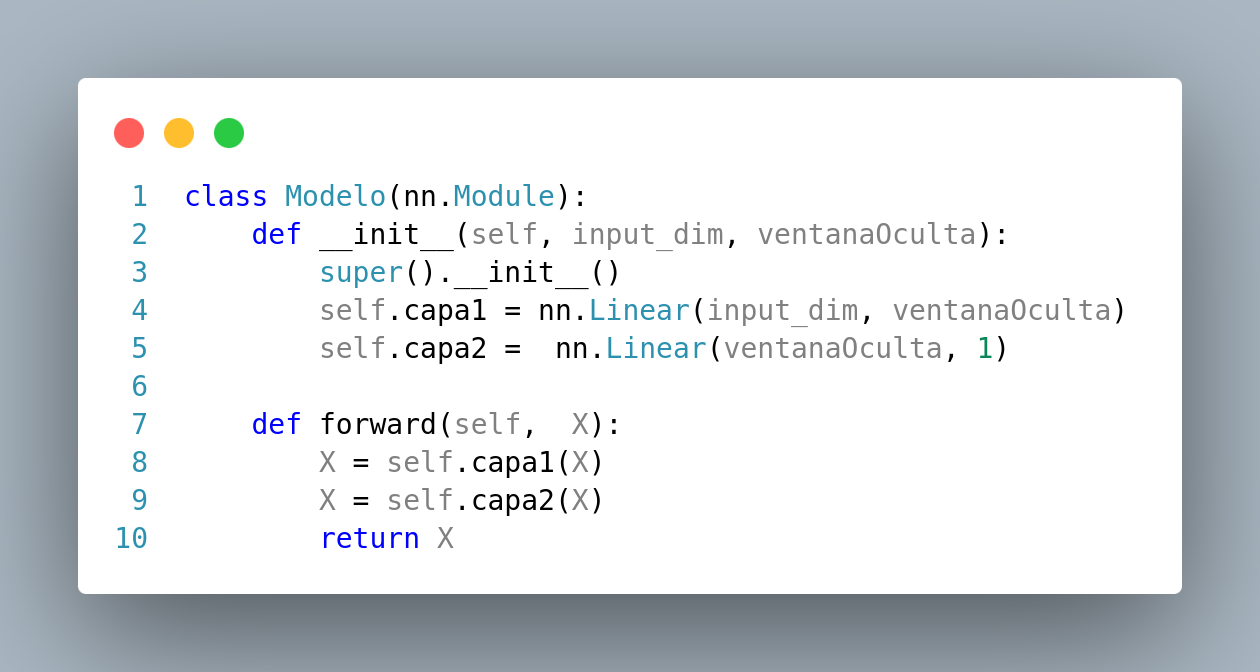
\includegraphics[width=0.6\textwidth]{../Memoria/img/modelo/codigo/modeloBIN.png}
	    	\caption{Definición de la clase del modelo de clasificación binaria.}
    		\label{fig:modBIN}
	\end{figure}
	
	\begin{table}[H]
		\centering 
		\resizebox{0.6\textwidth}{!}{
		\begin{tabular}{|c|c|}
		\hline
		\textbf{Hiperparámetro} & \textbf{Posibles valores} \\ \hline
		\textit{Batch size} & [2000, 10000, 15000, 20000] \\ \hline
		\textit{Learning rate} & [$10^{-2}$, $10^{-3}$, $10^{-4}$] \\ \hline
		Épocas & [10, 20, 30] \\ \hline
		\end{tabular}
		}
		\caption{Valores de los hiperparámetros utilizados en los experimentos del modelo de clasificación binaria.}
		\label{tab:hiperBIN}
	\end{table}
\end{frame}

\begin{frame}{Implementación del MCM}
	\begin{itemize}
		\item \textbf{Función de pérdida}: \texttt{CrossEntropyLoss}
		\item \textbf{Algoritmo de optimización}: \texttt{AdamW}
	\end{itemize}
	
	\begin{figure}[H]
	    \centering
	    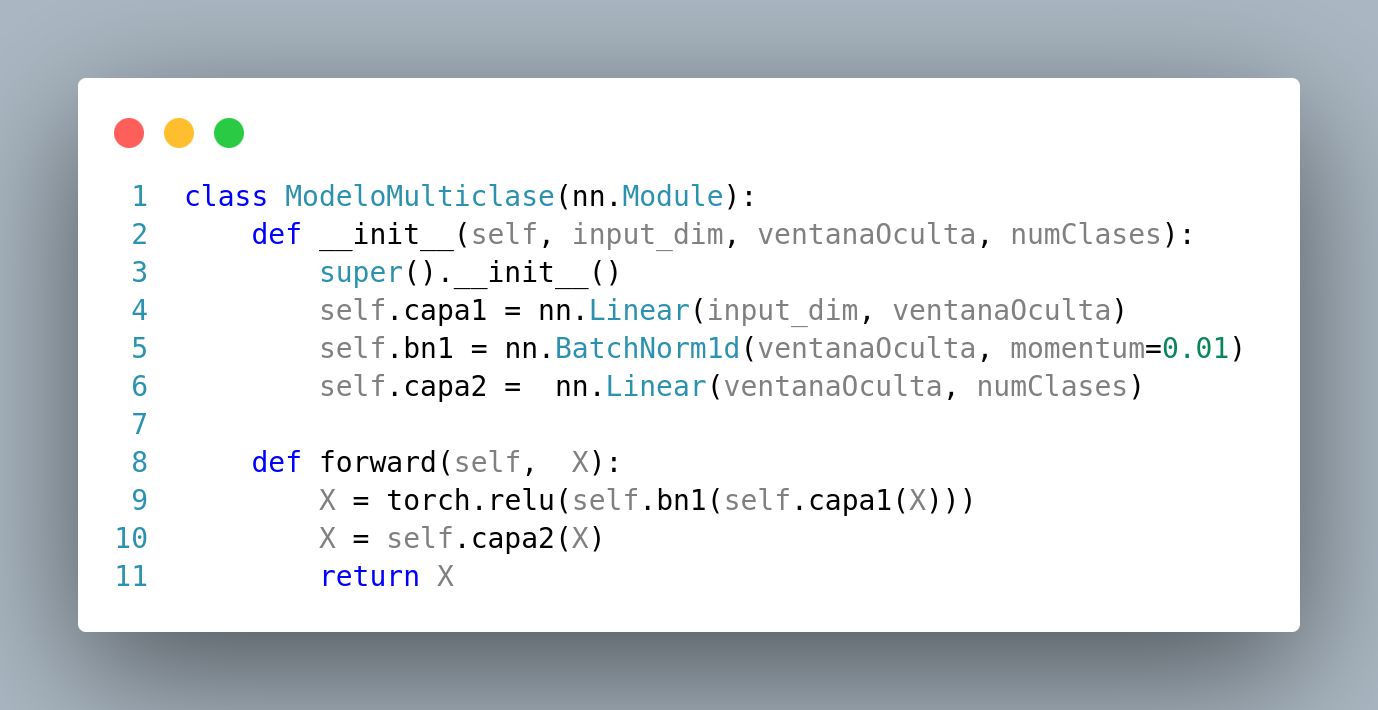
\includegraphics[width=0.6\textwidth]{../Memoria/img/modelo/codigo/modeloMUL.png}
	    	\caption{Definición de la clase del modelo de clasificación multiclase.}
    		\label{fig:modBIN}
	\end{figure}
	
	\begin{table}[H]
		\centering 
		\resizebox{0.6\textwidth}{!}{
		\begin{tabular}{|c|c|}
		\hline
		\textbf{Hiperparámetro} & \textbf{Posibles valores} \\ \hline
		\textit{Batch size} & [32, 64, 128, 256, 512] \\ \hline
		\textit{Learning rate} & [$10^{-2}$, $10^{-3}$, $10^{-4}$, $10^{-5}$] \\ \hline
		Épocas & [30, 50, 80, 100] \\ \hline
		\end{tabular}
		}
		\caption{Valores de los hiperparámetros utilizados en los experimentos del modelo de clasificación multiclase.}
		\label{tab:hiperBIN}
	\end{table}
\end{frame}



\subsection{Selección de las configuraciones de los modelos}

\begin{frame}{Selección de los mejores MCB}
Los mejores resultados del MCB los obtuvo la arquitectura con el doble de neuronas en su capa oculta que atributos de entrada tiene el modelo.
\begin{columns}[b]
\begin{column}{0.7\textwidth}
\begin{table}[H]
		\resizebox{1\textwidth}{!}{
\begin{tabular}{|>{\columncolor[HTML]{E0FFFF}}l|c|c|c|c|c|}
\hline
Posicion\_EXP & 1º-MCB98 & 2º-MCB98 & 3º-MCB98 & 4º-MCB98 & 5º-MCB98 \\
\hline
\cellcolor[HTML]{E0FFFF}batch\_size & \cellcolor[HTML]{66ffa8}20000 & \cellcolor[HTML]{66ffa8}10000 & \cellcolor[HTML]{66ffa8}15000 & \cellcolor[HTML]{66ffa8}15000 & \cellcolor[HTML]{66ffa8}10000 \\
\cellcolor[HTML]{E0FFFF}epochs & \cellcolor[HTML]{b1bafb}10 & \cellcolor[HTML]{b1bafb}30 & \cellcolor[HTML]{b1bafb}30 & \cellcolor[HTML]{b1bafb}10 & \cellcolor[HTML]{b1bafb}20 \\
\cellcolor[HTML]{E0FFFF}learning\_rate & \cellcolor[HTML]{f99595}$10^{-2}$ & \cellcolor[HTML]{f99595}$10^{-3}$ & \cellcolor[HTML]{f99595}$10^{-3}$ & \cellcolor[HTML]{f99595}$10^{-2}$ & \cellcolor[HTML]{f99595}$10^{-3}$ \\
\cellcolor[HTML]{E0FFFF}avg\_f1 & 0.998124 & 0.997941 & 0.997771 & 0.998015 & 0.997730 \\
\cellcolor[HTML]{E0FFFF}avg\_fn & 18.4 & 21.6 & 22 & 22.4 & 22.6 \\
\cellcolor[HTML]{E0FFFF}avg\_fp & 36.8 & 39 & 43.6 & 36 & 44.2 \\
\cellcolor[HTML]{E0FFFF}avg\_precision & 0.997501 & 0.997351 & 0.997039 & 0.997554 & 0.996999 \\
\cellcolor[HTML]{E0FFFF}avg\_recall & 0.998749 & 0.998531 & 0.998504 & 0.998477 & 0.998463 \\
\cellcolor[HTML]{E0FFFF}avg\_roc\_auc & 0.999781 & 0.999777 & 0.999776 & 0.999773 & 0.999777 \\
\cellcolor[HTML]{E0FFFF}avg\_tn & 344127.4 & 344125.2 & 344120.6 & 344128.2 & 344120 \\
\cellcolor[HTML]{E0FFFF}avg\_tp & 14686.2 & 14683 & 14682.6 & 14682.2 & 14682 \\
\hline
\end{tabular}
}
    \caption{Mejores cinco configuraciones para el MCB98.}
    \label{fig:BINhs98}
\end{table}
\end{column}

\begin{column}{0.3\textwidth}
\begin{figure}[H]
    \centering
    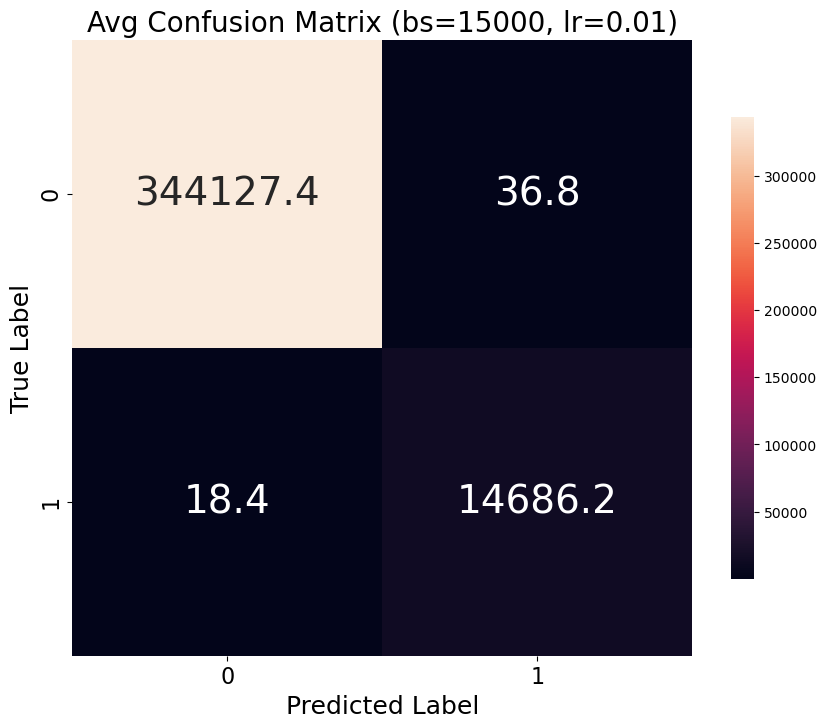
\includegraphics[width=1\textwidth]{../Memoria/img/modelo/matrices_confusion/MC_ENT_MCB98.png}
    \caption{Matriz de confusión 1º MCB98.}
    \label{fig:MC_ENT_MCB98}
\end{figure}

\end{column}
\end{columns}
\end{frame}


\begin{frame}{Mejores 5 configuraciones del MCB}
En este modelo no se observa que la arquitectura influya especialmente en los resultados obtenidos.
\begin{figure}[H]
    \centering
    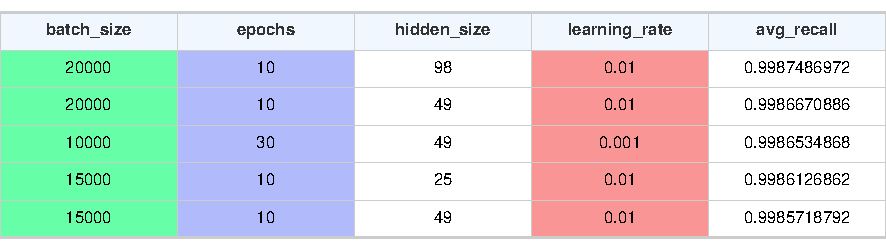
\includegraphics[width=0.85\textwidth]{../Memoria/img/modelo/resultados/BINtop5.pdf}
    \caption{Mejores cinco configuraciones de hiperparámetros del modelo de clasificación binaria.}
    \label{fig:BINtop5}
\end{figure}

\end{frame}




\begin{frame}{Selección de los mejores MCM}
Al igual que en el MCB, los mejores resultados del MCM se han obtenido en la arquitectura con el doble de neuronas en su capa oculta que atributos de entrada tiene el modelo.
\begin{columns}[b]
\begin{column}{0.7\textwidth}
\begin{table}[H]
		\resizebox{1\textwidth}{!}{
\begin{tabular}{|>{\columncolor[HTML]{E0FFFF}}l|c|c|c|c|c|}
\hline
Posicion\_EXP & 1º-MCM98 & 2º-MCM98 & 3º-MCM98 & 4º-MCM98 & 5º-MCM98 \\
\hline
\cellcolor[HTML]{E0FFFF}batch\_size & \cellcolor[HTML]{66ffa8}256 & \cellcolor[HTML]{66ffa8}256 & \cellcolor[HTML]{66ffa8}512 & \cellcolor[HTML]{66ffa8}64 & \cellcolor[HTML]{66ffa8}256 \\
\cellcolor[HTML]{E0FFFF}epochs & \cellcolor[HTML]{b1bafb}100 & \cellcolor[HTML]{b1bafb}80 & \cellcolor[HTML]{b1bafb}100 & \cellcolor[HTML]{b1bafb}80 & \cellcolor[HTML]{b1bafb}50 \\
\cellcolor[HTML]{E0FFFF}learning\_rate & \cellcolor[HTML]{f99595}$10^{-3}$ & \cellcolor[HTML]{f99595}$10^{-3}$ & \cellcolor[HTML]{f99595}$10^{-2}$ & \cellcolor[HTML]{f99595}$10^{-3}$ & \cellcolor[HTML]{f99595}$10^{-3}$ \\
\cellcolor[HTML]{E0FFFF}avg\_accuracy & 0.569414 & 0.556057 & 0.556915 & 0.556969 & 0.562083 \\
\cellcolor[HTML]{E0FFFF}avg\_f1\_macro & 0.413180 & 0.406773 & 0.388808 & 0.398720 & 0.397308 \\
\cellcolor[HTML]{E0FFFF}avg\_f1\_weighted & 0.583123 & 0.577553 & 0.574200 & 0.571020 & 0.569831 \\
\cellcolor[HTML]{E0FFFF}avg\_precision\_macro & 0.394898 & 0.385322 & 0.372836 & 0.377543 & 0.387029 \\
\cellcolor[HTML]{E0FFFF}avg\_precision\_weighted & 0.681971 & 0.675326 & 0.674534 & 0.669836 & 0.669688 \\
\cellcolor[HTML]{E0FFFF}avg\_recall\_macro & 0.577069 & 0.564962 & 0.573083 & 0.566046 & 0.550391 \\
\cellcolor[HTML]{E0FFFF}avg\_recall\_weighted & 0.569414 & 0.556057 & 0.556915 & 0.556969 & 0.562083 \\
\cellcolor[HTML]{E0FFFF}avg\_roc\_auc\_ovo & 0.813320 & 0.806782 & 0.809286 & 0.812789 & 0.800316 \\
\cellcolor[HTML]{E0FFFF}avg\_roc\_auc\_ovr & 0.788041 & 0.784984 & 0.781135 & 0.782758 & 0.777422 \\
\hline
\end{tabular}
}
    \caption{Mejores cinco configuraciones para el MCM98.}
    \label{fig:MULhs98}
\end{table}
\end{column}

\begin{column}{0.3\textwidth}
\begin{figure}[H]
    \centering
    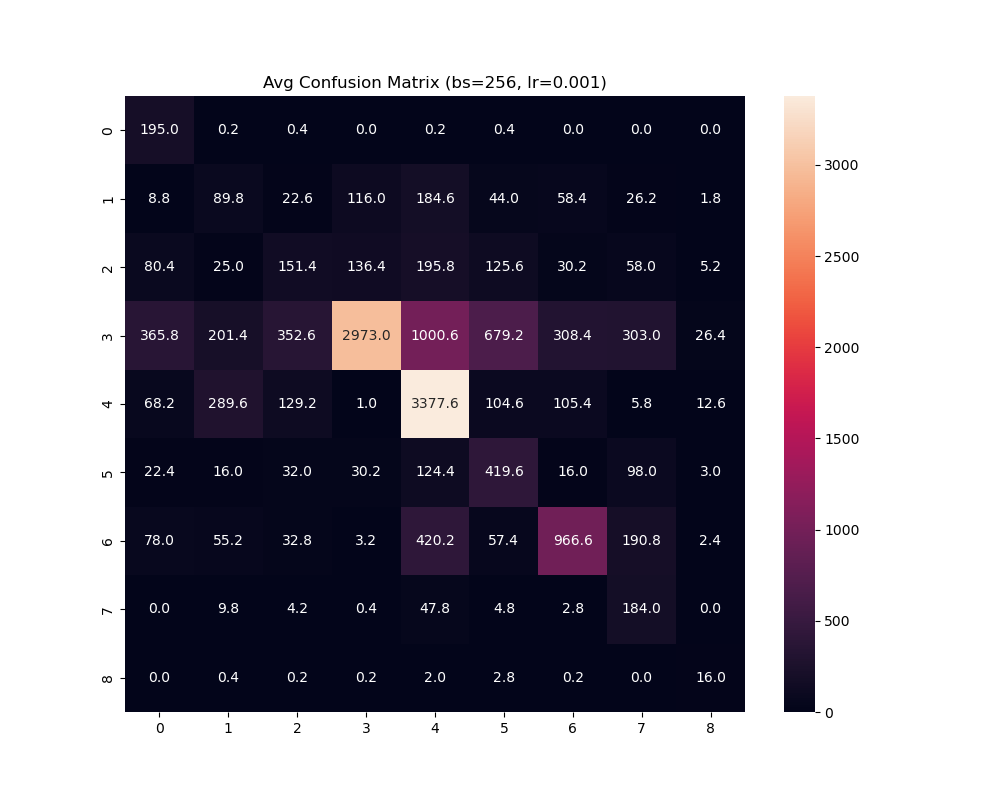
\includegraphics[width=1\textwidth]{../Memoria/img/modelo/matrices_confusion/MC_ENT_MCM98.png}
    \caption{Matriz de confusión 1º MCM98.}
    \label{fig:MC_ENT_MCM98}
\end{figure}

\end{column}
\end{columns}
\end{frame}


\begin{frame}{Mejores 10 configuraciones del MCM}
En el caso del MCM, la arquitectura MCM98 ha obtenido en la fase de entrenamiento unos resultados muy superiores a las otras dos arquitecturas desarrolladas.
\begin{figure}[H]
    \centering
    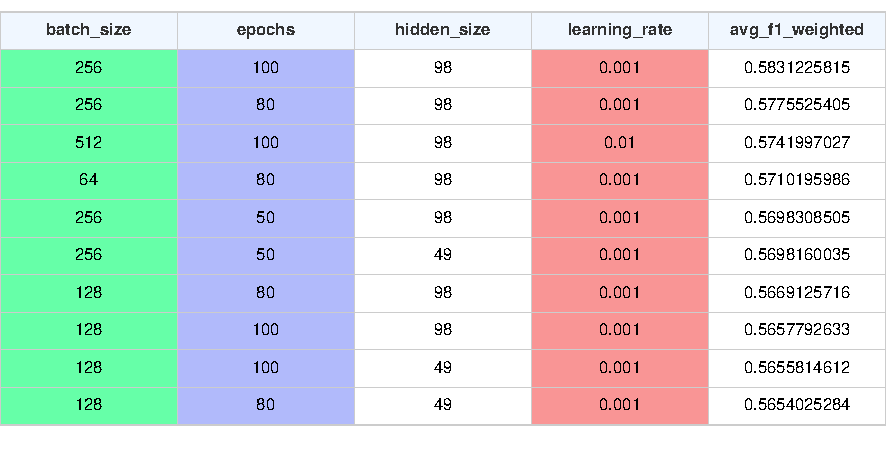
\includegraphics[width=1\textwidth]{../Memoria/img/modelo/resultados/MULtop10.pdf}
    \caption{Mejores diez configuraciones de hiperparámetros del modelo de clasificación multiclase.}
    \label{fig:BINtop5}
\end{figure}

\end{frame}






























\section{Evaluación}
Este capítulo se centra en la evaluación final de los modelos entrenados. Se describe el conjunto de datos de prueba, el proceso de evaluación, la presentación de los resultados de las métricas y el análisis de las fortalezas y debilidades de los modelos.

\section{Conjunto de datos de prueba}
Para obtener el conjunto de datos para el entrenamiento de los modelos y el conjunto de datos de prueba, se divide el conjunto total de los datos, una vez que estos han sido preparados como siguiendo los pasos que se comentan en la sección anterior \ref{sec.prep-datos} \nameref{sec.prep-datos}. 

Durante la división, es necesario estratificar los datos. Como se comenta en capítulos anteriores, la estratificación de los datos consiste en dividir el conjunto de datos de manera que se mantenga la misma distribución de clases en cada subconjunto. Esto es especialmente útil cuando las clases están desbalanceadas, asegurando que todos los subconjuntos tengan una representación proporcional de cada clase, lo que mejora la precisión del modelo y evita sesgos. Debido al desbalanceo que presentan los datos utilizados en este trabajo, es fundamental estratificarlos cada vez que se dividen para evitar que algunas particiones de los datos cuente solo con conexiones de una clase.

La división del conjunto de datos suele ser de en un 80\% para entrenamiento y un 20\% para evaluación, esta división se fundamenta en la necesidad de proporcionar suficiente cantidad de datos para que el modelo aprenda de manera efectiva, mientras se mantiene un conjunto de datos no utilizado en el entrenamiento para evaluar su rendimiento generalizado. La proporción del 80\% se considera adecuada para capturar patrones significativos en el entrenamiento sin comprometer la capacidad de evaluar el modelo en datos no vistos, lo que permite estimar su desempeño en situaciones realistas. Esta práctica también ayuda a evitar el sobreajuste, garantizando que los resultados del modelo no dependa en exclusiva de los datos utilizados en el entrenamiento \cite{bishop2006pattern}.

Para realizar la división, se utiliza la función \texttt{train\_test\_split} de la biblioteca \texttt{sklearn.model\_selection}. Esta función recibe el conjunto de los atributos y de las etiquetas de todo el \textit{dataset} utilizado, una vez que sus datos han sido preparados. Además, esta función recibe el porcentaje de los datos que se desea reservar para la evaluación o la fase de test, como se comenta en el párrafo anterior, en este trabajo el $0,2$ sobre 1 de los datos se destinan a evaluar los modelos entrenados. Finalmente, se especifica una semilla para que los datos se organicen de manera aleatoria y se especifica que se desea estratificar siguiendo el conjunto de las etiquetas.

Una vez divididos los datos, se normalizan los datos de evaluación, se convierten a tensores el conjunto de los atributos de pruebas y el conjunto de las etiquetas y se crea con estos tensores la instancia de la clase \texttt{DatasetTFG} que se utilizará para evaluar los modelos.

\section{Proceso de evaluación}
En el proceos de búsqueda de las configuraciones de hiperparámetros de los modelos con las que estos convergen mejor hacia una solución más generalizada, se utiliza la validación cruzada como se comenta en la sección \ref{subsec:conjdatent}. La validación cruzada se utiliza para encontrar los mejores hiperparámetros de un modelo debido a su capacidad para proporcionar una evaluación más robusta y confiable del rendimiento del modelo. Este método divide el conjunto de datos en varios subconjuntos, realizando múltiples entrenamientos y evaluaciones, lo que permite reducir el riesgo de sobreajuste a un subconjunto específico. Además, la validación cruzada maximiza el uso de los datos disponibles, lo que resulta especialmente útil cuando los datos son limitados. 

Una vez que se han encontrado los hiperparámetros óptimos, se utiliza todo el conjunto de datos de entrenamiento para entrenar los modelos finales. Esto se debe a que, al haber ajustado previamente los hiperparámetros, se considera que lso modelos se encuentran en sus configuraciones más eficientes, lo cual maximiza sus capacidades de generalización al aprender de la mayor cantidad de datos posible. De este modo, se obtienen unos modelos más robusto antes de realizar la evaluación final sobre un conjunto de prueba independiente que no ha sido utilizado en el proceso de entrenamiento \cite{hastie2009elements}.

El procesos de evaluación consiste en proporcionar a los modelos entrenados con las configuraciones comentadas en los párrafos anteriores, los datos de evaluación que no han visto durante la fase de entrenamiento. Durante este proceso, se recogen los resultados que se obtienen en función de la matriz de confusión correspondiente a cada modelo para posteriormente obtener las métricas con las que comparar el desempeño de los modelos.

\section{Resultados de las métricas en el proceso de evaluación}
Para comparar los resultados obtenidos en la fase de evaluación de las cinco mejores configuraciones de hiperparámetros de cada arquitectura de cada modelo, se utilizan las mismas métricas comentadas en las secciones \ref{sec.metricas-bin} \nameref{sec.metricas-bin} y \ref{sec:metricas-mul} \nameref{sec:metricas-mul} correspondientemente.

Con el objetivo de que la interpretación de los datos sea más sencilla, se ha añadido a las siguientes figuras una columna con la posición del \textit{ranking} que ocupó cada configuración en la fase anterior.




\subsection{Resultados del modelo de clasificación binaria}
La métrica utilizada para establecer el orden en los siguientes \textit{rankings} de configuraciones para los modelos de clasificación binaria es la misma empleada durante la fase previa de búsqueda de las mejores configuraciones de hiperparámetros: el \textit{Recall}.

\subsubsection{MCB25: Modelo de clasifcación binaria con un tamaño de capa oculta igual a la mitad del número de atributos de entrada que recibe el modelo}
En la Figura \ref{fig:EVALMCB25}, se muestran los resultados obtenidos durante las evaluaciones de las cinco configuraciones de hiperparámetros con mejor desempeño durante la fase de búsqueda de las mejores configuraciones para la arquitectura del modelo de clasificación binaria que posee un tamaño de capa oculta de 25 neuronas.

\begin{figure}[H]
    \centering
    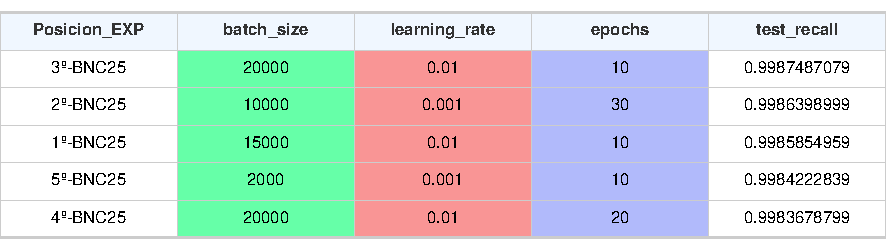
\includegraphics[width=0.9\textwidth]{./img/evaluacion/EVALMCB25.pdf}
    \caption{Resultados de la evaluación del modelo de  clasificación binaria con \textit{n/2} neuronas en la capa oculta siendo \textit{n} el número de atributos de entrada.}
    \label{fig:EVALMCB25}
\end{figure}

Los valores de la métrica \textit{Recall} obtenidos en las evaluaciones del modelo MCB25, son muy altos para todas las configuraciones y la diferencia entre sus valores es del orden de $1e-4$. Estas diferencias pueden deberse a circunstancias no controlables como el estado en el que se encontraba la máquina cuando se realizó la evaluación de los modelos o los pesos aleatorios iniciales que se eligieron en esa ejecución de los \textit{test}.

\subsubsection{MCB49: Modelo de clasifcación binaria con un tamaño de capa oculta igual al número de atributos de entrada que recibe el modelo}
En la Figura \ref{fig:EVALMCB49} se presentan los resultados obtenidos durante las evaluaciones de las cinco configuraciones de hiperparámetros con mejor desempeño, seleccionadas en la fase de búsqueda para la arquitectura del modelo de clasificación binaria que cuenta con una capa oculta de 49 neuronas.

\begin{figure}[H]
    \centering
    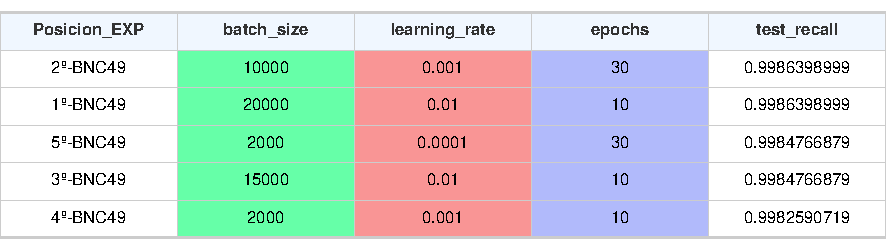
\includegraphics[width=0.9\textwidth]{./img/evaluacion/EVALMCB49.pdf}
    \caption{Resultados de la evaluación del modelo de clasificación binaria con \textit{n} neuronas en la capa oculta siendo \textit{n} el número de atributos de entrada.}
    \label{fig:EVALMCB49}
\end{figure}

Los valores de la métrica \textit{Recall} obtenidos durante las evaluaciones del modelo MCB49 son consistentemente altos para todas las configuraciones, y las diferencias entre ellos se encuentran en el orden de magnitud de $1e-4$. Estas variaciones podrían atribuirse a factores no controlables, como el estado del sistema al momento de la evaluación o la aleatoriedad en la inicialización de los pesos durante la ejecución de las pruebas.

\subsubsection{MCB98: Modelo de clasifcación binaria con un tamaño de capa oculta igual al doble del número de atributos de entrada que recibe el modelo}
La Figura \ref{fig:EVALMCB98} muestra los resultados obtenidos en las evaluaciones correspondientes a las cinco configuraciones de hiperparámetros que presentaron el mejor desempeño durante la fase de búsqueda, aplicadas a la arquitectura del modelo de clasificación binaria con una capa oculta de 98 neuronas.

\begin{figure}[H]
    \centering
    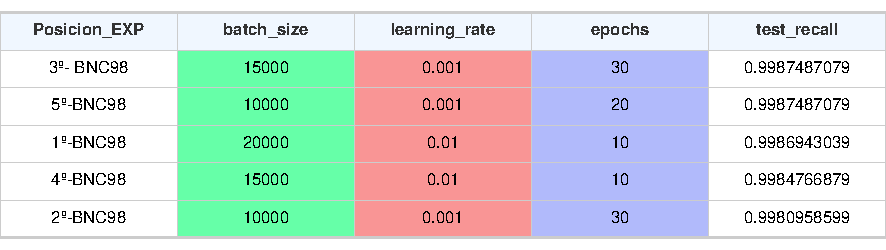
\includegraphics[width=0.9\textwidth]{./img/evaluacion/EVALMCB98.pdf}
    \caption{Resultados de la evaluación del modelo de clasificación binaria con \textit{2n} neuronas en la capa oculta siendo \textit{n} el número de atributos de entrada.}
    \label{fig:EVALMCB98}
\end{figure}

En las evaluaciones del modelo MCB98, los valores obtenidos para la métrica Recall fueron elevados en todas las configuraciones, con diferencias del orden de $1e-4$. Estas pequeñas variaciones pueden explicarse por factores no controlables, como el estado del sistema en el momento de la evaluación o la inicialización aleatoria de los pesos durante la ejecución de las pruebas.






\subsection{Resultados del modelo de clasificación multiclase}
Para determinar el orden de los \textit{rankings} presentados a continuación, se emplea la misma métrica utilizada en la fase anterior de búsqueda de configuraciones de hiperparámetros para los modelos de clasificación multiclase: el \textit{F1-weighted}.

\subsubsection{MCM25: Modelo de clasifcación multiclase con un tamaño de capa oculta igual a la mitad del número de atributos de entrada que recibe el modelo}

En la Figura \ref{fig:EVALMCM25} se presentan los resultados obtenidos durante las evaluaciones de las cinco configuraciones de hiperparámetros con mejor rendimiento, identificadas durante la fase de búsqueda para la arquitectura del modelo de clasificación multiclase que cuenta con una capa oculta de 25 neuronas.

\begin{figure}[H]
    \centering
    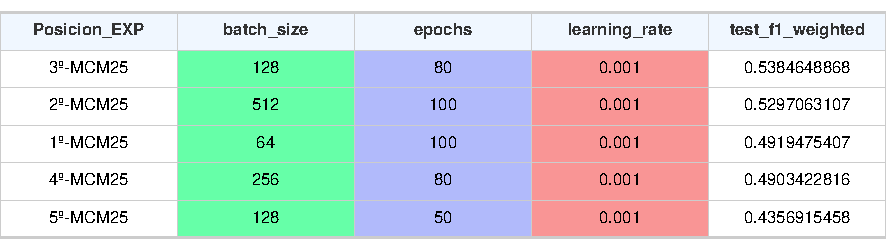
\includegraphics[width=0.9\textwidth]{./img/evaluacion/EVALMCM25.pdf}
    \caption{Resultados de la evaluación del modelo de clasificación multiclase con \textit{n/2} neuronas en la capa oculta siendo \textit{n} el número de atributos de entrada.}
    \label{fig:EVALMCM25}
\end{figure}

La figura anterior evidencia una diferencia en los valores de la métrica de comparación considerablemente mayor que la observada para las mismas configuraciones durante la fase de búsqueda de hiperparámetros. En los cinco mejores experimentos representados en la figura, las diferencias en la métrica \textit{F1-weighted} durante la fase de búsqueda se encuentran en el orden de $1e-2$, mientras que en la fase de evaluación alcanzan un orden de $1e-1$, lo que indica una degradación clara en el desempeño de esta arquitectura. 


\subsubsection{MCB49: Modelo de clasifcación multiclase con un tamaño de capa oculta igual al número de atributos de entrada que recibe el modelo}
La Figura \ref{fig:EVALMCM49} presenta los resultados de las evaluaciones realizadas sobre las cinco configuraciones de hiperparámetros con mejor desempeño, seleccionadas durante la fase de búsqueda aplicada a la arquitectura del modelo de clasificación multiclase con una capa oculta compuesta por 49 neuronas.

\begin{figure}[H]
    \centering
    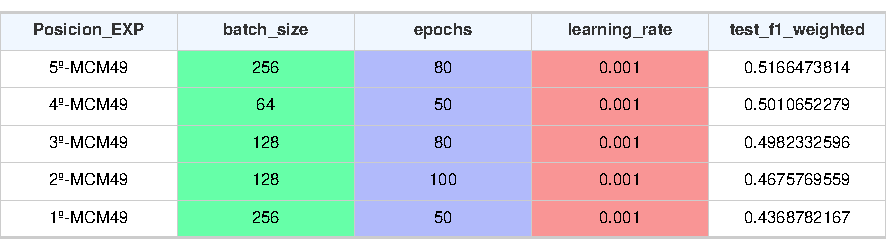
\includegraphics[width=0.9\textwidth]{./img/evaluacion/EVALMCM49.pdf}
    \caption{Resultados de la evaluación del modelo de clasificación multiclase con \textit{n} neuronas en la capa oculta siendo \textit{n} el número de atributos de entrada.}
    \label{fig:EVALMCM49}
\end{figure}

Al analizar los resultados obtenidos para esta arquitectura, destaca más allá del bajo rendimiento reflejado por la métrica \textit{F1-weighted}, el hecho de que el orden de las configuraciones se ha invertido respecto a lo observado en la fase de búsqueda. Las posibles causas de este comportamiento se detallan en la sección \ref{sec:analEVAL}.

\subsubsection{MCB98: Modelo de clasifcación multiclase con un tamaño de capa oculta igual al doble del número de atributos de entrada que recibe el modelo}
En la Figura \ref{fig:EVALMCM98} se ilustran los resultados obtenidos durante las evaluaciones correspondientes a las cinco configuraciones de hiperparámetros con mayor rendimiento, seleccionadas en la etapa de búsqueda de configuraciones para la arquitectura del modelo de clasificación multiclase con una capa oculta de 98 neuronas..

\begin{figure}[H]
    \centering
    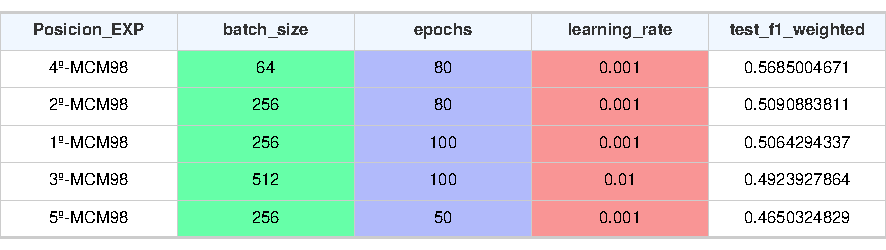
\includegraphics[width=0.9\textwidth]{./img/evaluacion/EVALMCM98.pdf}
    \caption{Resultados de la evaluación del modelo de clasificación multiclase con \textit{2n} neuronas en la capa oculta siendo \textit{n} el número de atributos de entrada.}
    \label{fig:EVALMCM98}
\end{figure}

Los resultados obtenidos durante la fase de evaluación de esta arquitectura fueron significativamente inferiores a los alcanzados en la fase de búsqueda. Por ejemplo, en la quinta mejor configuración de hiperparámetros, la diferencia entre los resultados experimentales y los obtenidos en la evaluación es del orden de $1e-1$. Esta diferencia implica una reducción del 10\% en la precisión, o bien, un mayor número de errores en las clases con menor cantidad de muestras en comparación con la fase anterior.

\section{Análisis de los resultados obtenidos} \label{sec:analEVAL}
\subsection{Modelo de clasificación binaria}

Los resultados obtenidos durante la fase de búsqueda de las mejores configuraciones de hiperparámetros, empleando validación cruzada \textit{k-fold} con estratificación, muestran valores de \textit{Recall} consistentemente altos, todos por encima de $0{,}9985$, como se detalla en la Figura \ref{fig:BINtop5}. Este rendimiento indica una capacidad del modelo para identificar correctamente la clase mayoritaria de forma fiable y robusta en distintos subconjuntos de datos, lo cual respalda la estabilidad de las configuraciones seleccionadas durante esta fase de optimización \cite{bergstra2012random}.

Sin embargo, al aplicar estas mismas configuraciones en la fase de evaluación sobre un conjunto independiente (Figura \ref{fig:top5EVALMCB}), se observa una inversión parcial en el orden del rendimiento de las configuraciones. Algunas de las configuraciones con mejor desempeño en la búsqueda no mantienen su posición, mientras que otras ascienden en el \textit{ranking}. Este comportamiento puede atribuirse a pequeñas variaciones aleatorias en los datos o a la sensibilidad del modelo frente a distribuciones ligeramente diferentes, aun cuando estas diferencias se hayan mitigado mediante estratificación \cite{reimers2017optimal}.

A pesar de que las diferencias absolutas entre los valores de \textit{Recall} en ambas fases son reducidas (del orden de $1e-4$ a $1e-3$), su impacto puede ser relevante en tareas de clasificación binaria crítica, como la detección de conexiones maliciosas, donde incluso mínimas variaciones pueden traducirse en decisiones erróneas. La ligera degradación observada en algunos casos puede deberse a factores como la inicialización aleatoria de pesos o el estado del sistema durante la inferencia, más que a un verdadero sobreajuste, dado que el proceso de validación cruzada ya controla adecuadamente este riesgo \cite{goodfellow2016deep}.

Asimismo, el análisis muestra que distintas combinaciones de \texttt{batch\_size}, \texttt{epochs}, \texttt{hidden\_size} y \texttt{learning\_rate} conducen a valores de \textit{Recall} muy próximos en evaluación. Esta convergencia en el rendimiento es coherente con estudios que sugieren que múltiples configuraciones en regiones planas del espacio de pérdida pueden llevar a modelos igualmente eficaces, especialmente en arquitecturas suficientemente expresivas como las utilizadas \cite{bouthillier2021sloppy}.

La observación de que varias configuraciones producen valores prácticamente idénticos de \textit{Recall} en la evaluación sugiere la presencia de una región de estabilidad en el espacio de soluciones. Sin embargo, el hecho de que estas configuraciones no coincidan con las mejor posicionadas en la búsqueda indica que, aunque la validación cruzada estratificada proporciona una estimación robusta, puede no capturar completamente la variabilidad inherente del conjunto de evaluación, especialmente si este presenta ligeras desviaciones de la distribución global \cite{recht2019imagenet}.

Los resultados reflejan un comportamiento coherente con lo esperado para modelos que han sido correctamente validados. Las diferencias encontradas entre fases no parecen ser estadísticamente significativas, pero sí lo suficientemente marcadas como para sugerir la conveniencia de utilizar estrategias complementarias de evaluación en futuros experimentos, como pruebas de sensibilidad o análisis de varianza.

\begin{figure}[H]
    \centering
    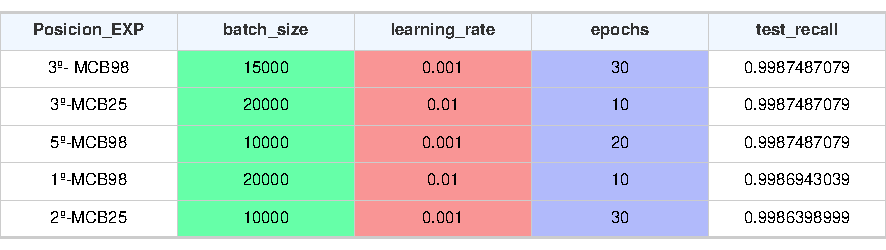
\includegraphics[width=0.9\textwidth]{./img/evaluacion/top5EVALMCB.pdf}
    \caption{Mejores cinco modelos en la fase de evaluación del modelo de clasificación binaria.}
    \label{fig:top5EVALMCB}
\end{figure}

\subsection{Modelo de clasificación multiclase}

Los resultados obtenidos durante la fase de búsqueda de hiperparámetros del modelo de clasificación multiclase (MCM), reflejados en la Figura \ref{fig:MULtop10}, indican valores moderados en las métricas utilizadas. En particular, el valor promedio de \textit{F1-weighted} se sitúa en torno a $0{,}57$, con ligeras variaciones entre las distintas configuraciones probadas. Este nivel de desempeño es coherente con la naturaleza desbalanceada del conjunto de datos, ya que el predominio de algunas clases afecta negativamente al promedio ponderado de precisión y \textit{Recall} \cite{he2009learning}.

Las métricas \textit{F1-macro} y \textit{Precision-macro} presentan valores sustancialmente más bajos que sus contrapartes ponderadas, lo que confirma que el modelo no logra un rendimiento equilibrado entre clases minoritarias y mayoritarias. Esta brecha sugiere que las clases menos representadas no son detectadas con suficiente eficacia, un fenómeno frecuente en escenarios de desbalance como el que se presenta en este trabajo, incluso al aplicar validación cruzada estratificada \cite{johnson2019survey}.

Al observar los resultados de la fase de evaluación (Figura \ref{fig:top5EVALMCM}), se constata que la métrica \textit{F1-weighted} no mejora significativamente respecto a la fase de búsqueda. De hecho, se observan valores incluso más bajos en algunas configuraciones, con un máximo de aproximadamente $0{,}568$ y un mínimo cercano a $0{,}509$. Este comportamiento sugiere que las configuraciones seleccionadas no generalizan adecuadamente al conjunto completo, a pesar de haber sido validadas mediante \textit{k-folds} \cite{reimers2017optimal}.

El análisis también muestra que el orden de las configuraciones en términos de rendimiento cambia entre ambas fases. Configuraciones que ocupaban posiciones intermedias o bajas durante la búsqueda escalan posiciones en la evaluación y viceversa. Esto podría estar relacionado con la distribución específica de las clases en el conjunto completo usado para la evaluación, el cual puede no coincidir exactamente con la distribución estratificada de los pliegues empleados durante la validación por circunstancias no controlables \cite{buda2018systematic}.

La pérdida de rendimiento observada puede explicarse también por el hecho de que, al entrenar con el conjunto completo en la evaluación, se pierde la ventaja del promedio sobre múltiples particiones que ofrece la validación cruzada. Esta situación puede inducir mayor varianza en los resultados y resaltar la sensibilidad del modelo a configuraciones particulares del entrenamiento \cite{dietterich1998approx}.

Por otra parte, el hecho de que el mejor resultado de \textit{F1-weighted} en evaluación ($0{,}568$) sea comparable al mejor valor obtenido en la búsqueda sugiere que el modelo alcanza un rendimiento máximo limitado por la naturaleza del problema. La estructura altamente desbalanceada del conjunto impone un techo al rendimiento global del modelo \cite{japkowicz2002class}.

El modelo de clasificación multiclase presenta un rendimiento aceptable dadas las condiciones desbalanceadas del problema, pero revela claras limitaciones en la detección equilibrada de clases. Las discrepancias entre búsqueda y evaluación reflejan la dificultad del modelo para mantener un rendimiento robusto al exponerse a la totalidad del conjunto, y sugieren la necesidad de introducir nuevas estrategias no probadas en la sección \ref{subsec:MCMdescart} \nameref{subsec:MCMdescart} orientadas al tratamiento explícito del desbalanceo de clases en futuras fases del desarrollo.

\begin{figure}[H]
    \centering
    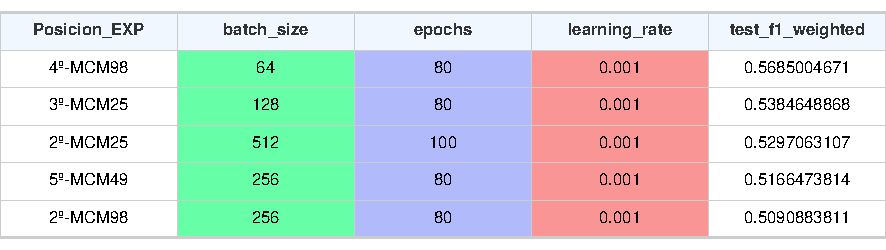
\includegraphics[width=0.9\textwidth]{./img/evaluacion/top5EVALMCM.pdf}
    \caption{Mejores cinco modelos en la fase de evaluación del modelo de clasificación multiclase.}
    \label{fig:top5EVALMCM}
\end{figure}



\section{Despliegue}
\begin{frame}{Despliegue de los modelos en un entorno real}
El despliegue efectivo de estos modelos contribuye a mejorar la seguridad en redes mediante la automatización de la detección de conexiones malignas, permitiendo respuestas rápidas y reducidir el número de falsos positivos y negativos. La diferenciación entre múltiples tipos de conexiones malignas aporta un valor añadido para estrategias de mitigación específicas y optimización de recursos.

\begin{figure}[H]
    \centering
    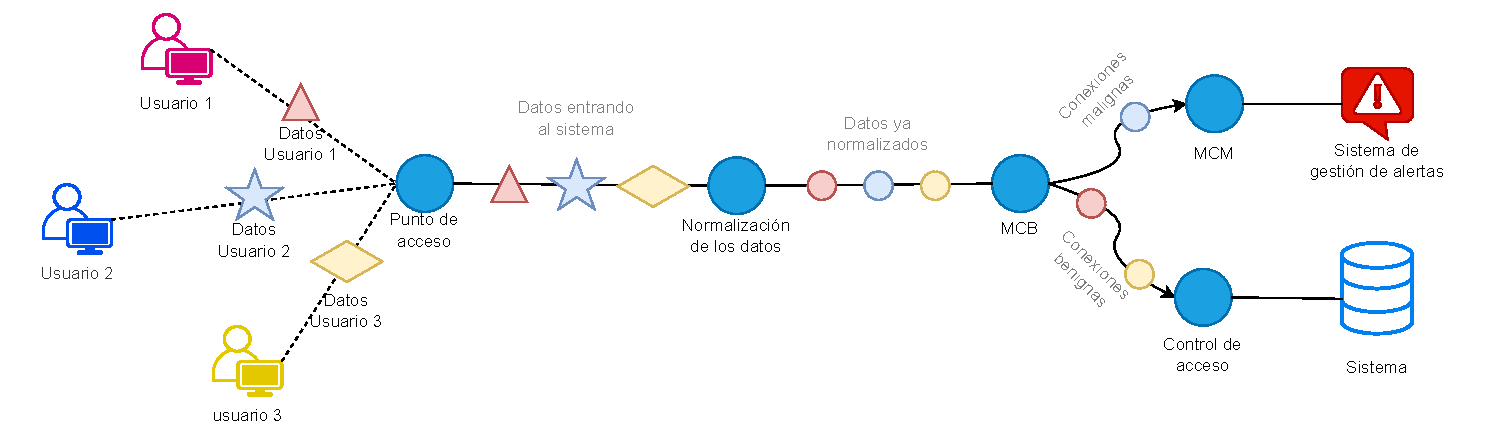
\includegraphics[width=1\textwidth]{../Memoria/img/despliegue/despliegue.pdf}
    \caption{Ejemplo de despliegue de los modelos en un sistema informático.}
    \label{fig:despliegue}
\end{figure}

\end{frame}

\section{Conclusiones}

En este capítulo se exponen las conclusiones derivadas del desarrollo y evaluación del modelo neuronal diseñado para la clasificación de conexiones benignas y malignas. El enfoque propuesto consiste en un modelo de clasificación binaria que, una vez realiza la distinción entre conexiones benignas y malignas, redirige aquellas conexiones clasificadas como malignas hacia un modelo de clasificación multiclase. Este último modelo es capaz de diferenciar las conexiones malignas en nueve clases distintas, permitiendo una identificación más detallada y precisa de los diversos tipos de intrusiones. Los resultados obtenidos destacan la eficacia de ambos modelos, evidenciando su capacidad para abordar de manera jerárquica y especializada la clasificación. Finalmente, se presentan las limitaciones del estudio y se plantean posibles líneas de trabajo futuro.

\section{Conclusiones}

El primer objetivo del proyecto, consistente en diseñar e implementar un modelo capaz de detectar intrusiones en redes informáticas y proporcionar una clasificación preliminar de las mismas, se ha cubierto de forma satisfactoria. Este primer objetivo del proyecto se ha alcanzado al obtener un modelo de clasificación binaria capaz de distinguir entre conexiones benignas y malignas con un \textit{Recall} superior a $0.99$. Con respecto a la clasificación de intrusiones o conexiones malignas, se ha desarrollado un modelo de clasificación multiclase, que recibe las conexiones clasificadas por el modelo binario como malignas y clasifica estas conexiones en nueve clases diferentes de intrusiones en sistemas informáticos con un \textit{F1-weighted} cercano a $0.6$.

El segundo objetivo del proyecto, según el cual los modelos de detección debían ser modelos neuronales, se ha alcanzado satisfactoriamente. Este objetivo se logró mediante el diseño de modelos de clasificación binaria (MsCB) y multiclase (MsCM), ambos con una arquitectura compuesta por dos capas. La primera de las capas en todos los modelos corresponde con la capa oculta, es la capa que recibe los atributos de entrada del modelo y la que permite que se pueda resolver el problema no lineal que se propone en este trabajo. Esta primera capa cuenta con un número diferente de neuronas en función de la arquitectura del modelo que se observe. La segunda capa por su parte, es la que corresponde con la salida del modelo. Esta segunda capa cuenta con una única neurona en el caso de los MsCB y con nueve neuronas en el caso de los MsCM.  La utilización de un Perceptrón Multicapa (MLP) en ambos modelos de clasificación permite aprovechar la capacidad de las redes neuronales para aprender representaciones complejas y no lineales, mejorando la capacidad de clasificación

El tercer objetivo del proyecto, consistente en evaluar y comparar los modelos generados utilizando un conjunto de datos real y complejo, se ha alcanzado de manera adecuada. Tal y como se expone en el Capítulo \ref{cap.ent-datos}, correspondiente a la fase de entendimiento de los datos de la metodología CRISP-DM, el conjunto de datos empleado para dicha evaluación ha sido el \texttt{NF-UNSW-NB15-v3}. \cite{luay2025NetFlowDatasetsV3}. Este conjunto de datos es semi-sintético, esto se debe a que los flujos benignos son registros reales de la conexión entre dos sistemas, mientras que los flujos correspondientes a los ataques se generaron en un entorno controlado. Para evitar que los datos sintéticos de los flujos maliciosos perjudicasen el entrenamiento y la evaluación de los modelos, se transformaron los datos, eliminando aquellos atributos que presentaban valores que diferían con la realidad, como fue el caso de las direcciones IP.

Evaluar el grado en el que se han alcanzado los objetivos académicos es más complejo que evaluar si los objetivos del proyecto se han conseguido cumplir. Esta diferencia se debe a que mientras que los objetivos del proyecto son medibles cuantitativamente, los objeticos académicos no son medibles objetivamente. Sin embargo, teniendo en cuenta el trabajo desarrollado se considera que si se han alcanzado todos los objetivos académicos fijados.

El primer objetivo académico, centrado en comprender el funcionamiento de los modelos neuronales mediante \texttt{PyTorch} y las métricas de evaluación, se ha abordado a lo largo del desarrollo del proyecto. Al haber desarrollado varios modelos con difertes arquitecturas y calcular las métricas tanto de la fase de validación como de la fase de evaluación utilizando la biblioteca \texttt{PyTorch}, se puede afirmar que se ha comprendido el funcionamiendo de los modelos neuronales, alcanzando de esta manera el primer objetivo académico.

El segundo objetivo académico, consiste en aprender las características de varios de los tipo de modelos neruonales que existen, se ha alcanzado de manera satisfactoria. En la sección \ref{subsec.tiposmodel} del capítulo \ref{cap.modelos}, se explican algunos de los modelos neuronales que más se utilizan en la actualidad y se comentan las caracterísitcas de cada tipo de modelo, proporcionando una visión de las tareas en las que mejor desempeño muestra cada tipo. Tras analizar las características de los diferentes tipos de modelos neuronales, se determinó que el Perceptrón Multicapa (MLP) era la opción más adecuada para este problema, dado que los datos presentan una naturaleza no lineal y el MLP tiene la capacidad de aprender representaciones complejas y no lineales, lo cual resulta fundamental para resolver este tipo de clasificación. Para redactar la sección mencionada fue necesario entender cuales eran las caraterísticas de cada tipo de modelo neuronal, por lo que el segundo objetivo académico se ha cumplido correctamente durante el desarrollo de este trabajo.

El tercer objetivo académico, se centra en descubrir el potencial de las redes neuronales para optimizar y mejorar las tecnologías de la información, incluyendo la ciberseguridad de los sistemas, se ha cubiertod de manera satisfactoria . Tras el desarrollo de este trabajo se ha descubierto que los modelos neuronales tienen una gran capacidad para resolver problemas de clasificación con una complejidad elevada. Además, resulta fascinante el hecho de que los pesos de las neuronas se puedan ajustar en cualquier momento para converger hacia una solución más generalizada o precisa del problema. Esta capacidad de adaptación es esencial en las tecnologías de la información, y en especial en la ciberseguridad ya que es un campo que se encuentra en constante evolución. Teniendo esto en cuenta, no solo se ha descubierto el potencial de las redes neuronales para optimizar y mejorar las tecnologías de la información, incluyendo la ciberseguridad de los sistemas, si no que además se ha descubierto el potencial que tienen las redes neuronales para resolver problemas complejos y su alta capacidad de adaptación a cambios en el problema que resuelven.

%Puesto que se han completado todos los objetivos del proyecto, así como los objetivos académicos fijados al comienzo de la memoria, se puede afirmar que el trabajo ha sido un éxito. Se ha desarrollado un modelo capaz de detectar intrusiones en sistemas informáticos y clasificarlas en nueve tipos diferentes de intrusiones. Además, se han obtenido conocimientos acerca de las redes neuronales que se ignoraban por parte del alumno antes del desarrollo de este trabajo.


\section{Trabajo futuro}
En un posible trabajo futuro se podría explorar como afecta el uso de las técnicas que se comentan en esta sección en la eficacia y en la eficiencia de los modelos desarrollados, con el objetivo de obtener modelos que convejan hacia una solución que generalice mejor, especialmente en el modelo de clasificación multiclase.

\begin{itemize}
	\item Modificar la arquitectura del modelo de clasificación multiclase. Durante el desarrollo del trabajo se han comparado los resultados que se obtenían al modificar el tamaño de la capa oculta. Estas comparaciones han demostrado que en función de la complejidad del problema aumentar el número de neuronas puede ser beneficioso o contraproducente. También se ha probado a añadir una tercera capa en el modelo de clasificación multiclase para comprobar si aplicando esta técnica, el modelo conseguía compensar el desbalanceo en el número de muestras de algunas clases del conjunto de datos con la complejidad de la red neuronal. Desafortunadamente, el valor más alto obtenido en la métrica \textit{F1-weighted} utilizando una arquitectura de tres capas, no superó los resultados obtenidos por los modelos con dos capas.
	
	Sin embargo, al modificar la arquitectura del modelo de clasificación multiclase, sería posible lograr que el modelo converja hacia una solución que sea capaz de identificar con una mayor exactitud aquellas clases con un menor número de muestras, mejorando de esta manera la probabilidad de identificar tanto las clases minoritarias como las mayoritarias.
	
	\item Balancear las clases que identifica el modelo de clasificación multiclase añadiendo nuevos datos al conjunto de datos utilizado durante la fase de entrenamiento. Como se ha comentado en varias ocasiones, el conjunto de datos utilizado durante el entrenamiento de los modelos tiene una proporción realista entre los datos de las conexiones que lo conforman. Que el conjunto de datos presente esta característica es fundamental para comprobar cual sería el comportamiento del modelo en un entorno de producción real. El aspecto negativo, es que en la realidad no existe un equilibrio entre los tipos de intrusiones que sufre un sistema informático, por lo que los datos se encuentran extremadamente desbalanceados.
	
	Al utilizar datos balanceados durante la fase de entrenamiento del modelo y datos realistas durante la fase de evaluación del mismo, se obtendría un modelo capaz de distinguir mejor entre las nueve clases de intrusiones que se tratan en este trabajo y se podría comprobar la eficacia real del modelo de clasificación multiclase al evaluarlo con un conjunto de datos que representan de manera más fideligna las intrusiones que puede sufir un sistema informático.
	
	\item Desplegar los modelos para integrarlos en entornos operativos. Tal y como se comenta en el capítulo \ref{cap.despliegue}, desplegar los modelos contribuiría a mejorar la seguridad en redes mediante la automatización de la detección de conexiones malignas, como sucede con los IDS. Una vez detectada la actividad maliciosa, se podría dar respuestas rápidas a las intrusiones para mitigar sus efectos, como hacen los IPS.
	
	\item Entenar los modelos con los datos que estos reciben una vez desplegados. En las secciones anteriores se comenta que una de las ventajas de utilizar modelos neuronales para la detección de intrusiones en vez de algoritmos, es la capacidad de los modelos de aprender de las conexiones que reciben mientras están en producción y su potencial para detectar patrones no lineales que pueden presentar nuevos tipos de ataques desconocidos como los \textit{zero day}.
	
	\item Comparar los resultados obtenidos con los resultados de articulos publicaciones que utilicen el mismo \textit{dataset} o traten el tema de manera similar. Contrastar los resultados obtenidos con estudios previos que emplean el mismo dataset o abordan problemáticas similares permite evaluar objetivamente el desempeño del enfoque propuesto. Esta práctica no solo aporta rigor científico al análisis, sino que también facilita la identificación de avances, limitaciones y oportunidades de mejora en relación con investigaciones existentes.
\end{itemize}




\begin{frame}
\begin{center}
        {\Huge Muchas gracias por su atención.}
    \end{center}
    \begin{figure}[H]
        \begin{center}
            
\includegraphics[width=0.25\linewidth]{img/uva.eps}
        \end{center}
    \end{figure}

\end{frame}

\end{document}